
\documentclass[review,3p,times,authoryear,12pt]{elsarticle}



\usepackage{subfigure}
\usepackage{amsmath, amsthm, amssymb}

\usepackage{graphicx}
\usepackage{algorithm}
\usepackage{algorithmic}
\usepackage{clrscode3e}
\usepackage{url}
\usepackage{multirow}
\usepackage{longtable}
\usepackage{color}


\journal{Omega}
\newtheorem{corollary}{Corollary}
\newtheorem{theorem}{Theorem}
\newtheorem{definition}{Definition}
\newtheorem{proposition}{Proposition}
\newtheorem{lemma}{Lemma}
\begin{document}
\graphicspath{{./figure/}}
\begin{frontmatter}
\newpage

\title{Target-guided algorithms for the container pre-marshalling problem}

\author[shu]{Ning Wang}
\ead{wangning@cityu.edu.hk}

\author[cityu]{Bo Jin\corref{corl}}
\ead{msjinbo@cityu.edu.hk}

\author[nju]{Andrew Lim\fnref{lim}}
\ead{alim.china@gmail.com}

\address[shu]{
Department of Information Management, School of Management, Shanghai University, Shanghai, China
}

\address[cityu]{
Department of Management Sciences, City University of Hong Kong, Kowloon Tong, Hong Kong
}

\address[nju]{International Center of Management Science and Engineering, School of Management and Engineering, Nanjing University, Nanjing, Jiangsu, China}

\cortext[corl]{Corresponding author. Tel: +852 3442 5296}
\fntext[lim]{Andrew Lim is currently on no pay leave from City University of Hong Kong.}


\begin{abstract}
The container pre-marshalling problem (CPMP) aims to rearrange containers in a bay with the least movement effort; thus, in the final layout, containers are piled according to a predetermined order.
Previous researchers, without exception, assumed that all the stacks in a bay are functionally identical.
Such a classical problem setting is reexamined in this paper.
Moreover, a new problem the CPMP with a dummy stack (CPMPDS), is proposed.
At terminals with transfer lanes, a bay includes a row of ordinary stacks and a dummy stack.
The dummy stack is actually the bay space that is reserved for trucks.
Therefore, containers can be shipped out from the bay.
During the pre-marshalling process, the dummy stack temporarily stores containers as an ordinary stack.
However, the dummy stack must be emptied at the end of pre-marshalling.
In this paper, target-guided algorithms are proposed to handle both the classical CPMP and new CPMPDS.
All the proposed algorithms guarantee termination.
Improved lower bounds for the CPMP and CPMPDS are also devised.
Experimental results in terms of the CPMP show that the proposed algorithms surpass the state-of-the-art algorithm.
\end{abstract}

\begin{keyword}
container pre-marshalling \sep target-guided algorithms\sep lower bound \sep dummy stack
\end{keyword}
\end{frontmatter}

\section{Introduction}

Seaborne transportation is the cornerstone of international trade and undoubtedly an engine of global economic development.
According to the \textit{Review of Maritime Transport} (2012) released by the United Nations Conference on Trade and Development, approximately 80\% of global trade by volume is carried by sea.
Among different ship types, container ships account for approximately 62\% of dry cargoes.
Since the commencement of containerization, containers facilitate smooth flow of goods across multiple transportation modes without direct freight handling during the course of shipping.
Accompany with the rapid growth of container shipping, container terminals face unprecedented development opportunities.
The role of container terminals lies in providing physical spaces for container exchanges between sea and land.
At terminals, a large proportion of land spaces (known as container yards or warehouses) are reserved for storing containers temporarily.
A yard acts as a cache that ensures rapid loading and unloading of vessels.
Basically, a conventional practice of exporting containers is to store them on the yard first.
When vessels arrive, containers are transported by trucks to the quayside and then loaded onto vessels.
The process is reverse for importing containers.

High efficiency is a key factor for successful terminals because shipping line managers prefer efficient terminals.
Carriers or shippers bear the pressure of quick delivery from downstream customers.
Moreover, high efficiency increases the turnover rate of terminals and therefore generates more profit for shareholders.
Container terminals have every reason to increase their operational efficiency.
Terminal practitioners and operations researchers have paid considerable attention to improving the efficiency of quayside operations.
Nonetheless, overall terminal productivity will not increase dramatically if only quayside operations are optimized, thereby leaving yard operations inefficient \citep{Jiang2012}.

A yard is generally divided into several blocks.
A block is composed of several parallel bays.
Each bay is formed by several stacks aligned side by side.
In each stack, containers are piled vertically.
Figure \ref{fig:1} shows a diagram of a yard.
The height of stacks is constrained by the height of the operating equipment.
One stack can typically store 3 to 10 containers.

\begin{figure*}[!htb]
\centering
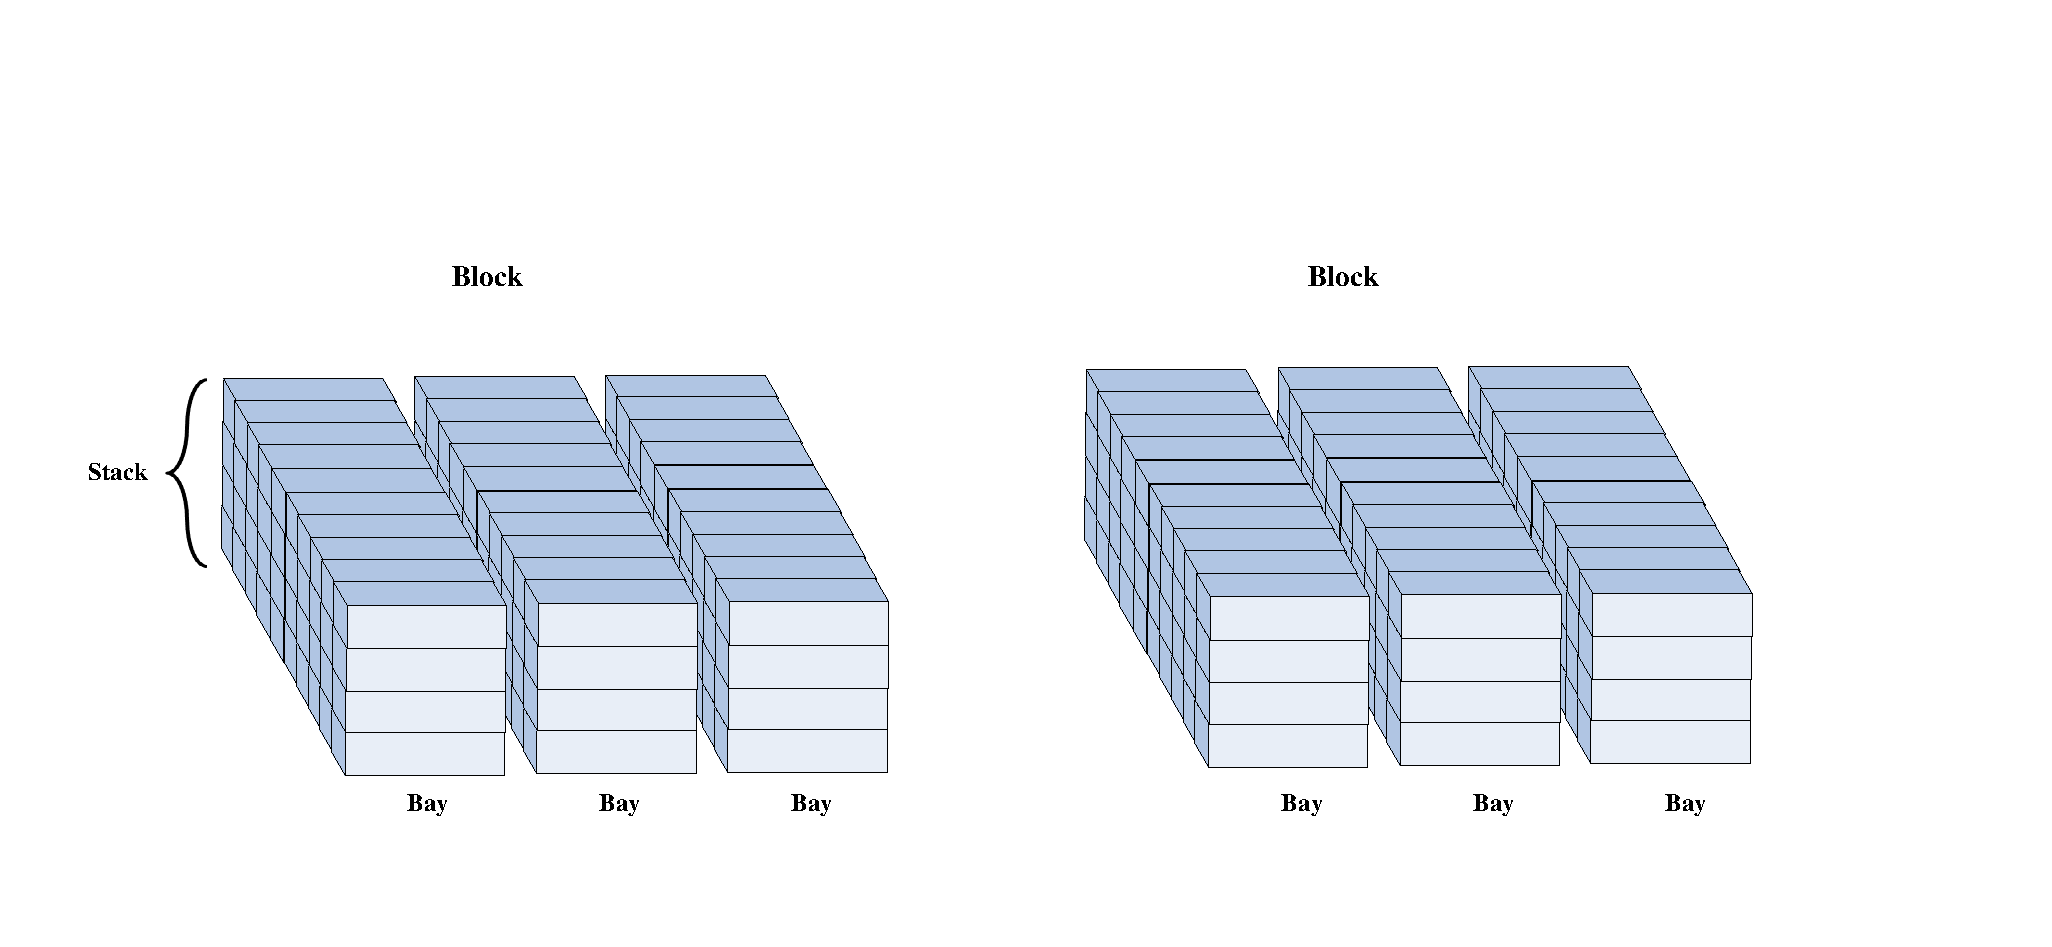
\includegraphics[width=0.7\textwidth]{fig1.pdf}
\caption{An example of a container yard}
\label{fig:1}
\end{figure*}

Containers in the same stack can only be retrieved in a ``first in, last out'' manner.
If the container to be fetched is not at the top of a stack, all the containers placed above it have to be relocated to other stacks before retrieving it.
Such forced movements are known as rehandles.
Container rehandle is costly because this additional task decreases the efficiency of container retrieval, but consignors do not pay for this task.
In the ideal situation, containers are piled in an order that is consistent with the retrieval order, i.e., containers retrieved earlier are located at higher tiers.
However, the practical situation does not always match the ideal wish.
The placement order of containers is decided by inland transportation or consignors, whereas the retrieval order of containers is decided by stowage planning or ship schedules. In most situations, the two orders are not exactly reverse. In reality, containers that arrive early do not necessarily depart late.

Prior to ship arrival, containers in a bay can be rearranged to comply with their retrieval order.
This process is called pre-marshalling.
Although it is not billable to consignors, pre-marshalling can reduce ship berthing time and increase terminal turnover rate.
Performing container pre-marshalling with the least effort is denoted as the container pre-marshalling problem (CPMP).

Although the CPMP has been studied, practical scenarios have not been fully depicted.
For terminals that use gantry cranes, there exist two kinds of I/O layouts where trucks and gantry cranes exchange containers \citep{Carlo2014}.
Figure \ref{fig15} shows the difference of two layouts.
In the first layout, I/O points form lanes (transfer lane) which are parallel to a block, while in the second layout, I/O points form bays which are at both ends of a block.
In the first layout, when no container is being retrieved, transfer lanes act as temporary stacks for the pre-marshalling work as ordinary stacks.
The only issue that demands attention is that transfer lanes should be empty after the pre-marshalling work, which distinguish themselves from ordinary stacks.
Transfer lanes are called \textbf{dummy stacks}.

\begin{figure}[!htb]
\centering
\subfigure[Layout with transfer lanes]{
    \label{fig15:1}
    \resizebox{0.25 \textwidth}{!}{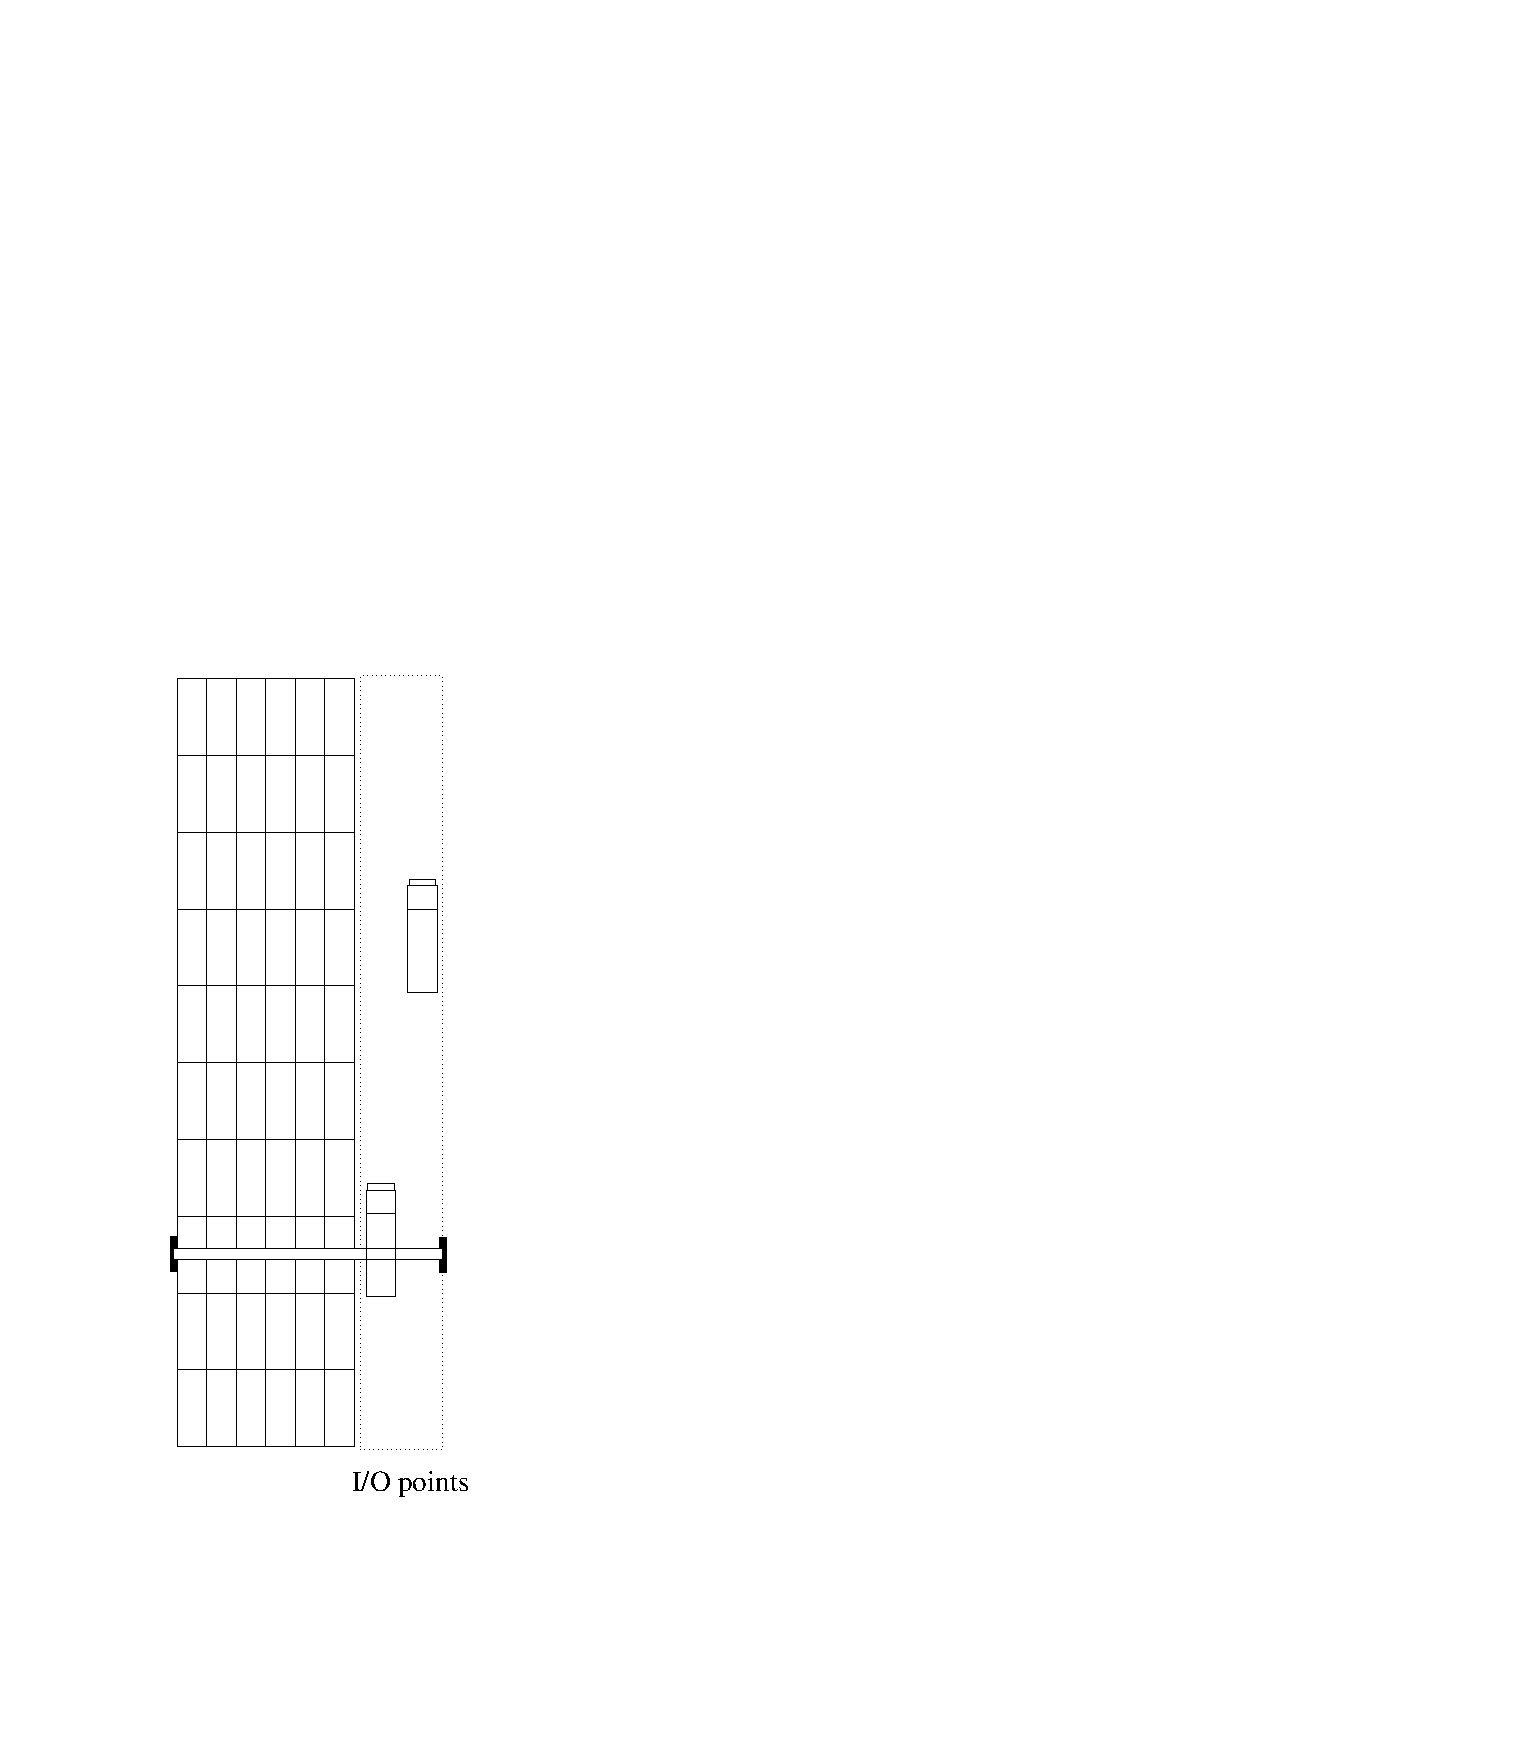
\includegraphics{fig15_1.pdf}}}
\subfigure[Layout with transfer bays]{
    \label{fig15:2}
    \resizebox{0.25 \textwidth}{!}{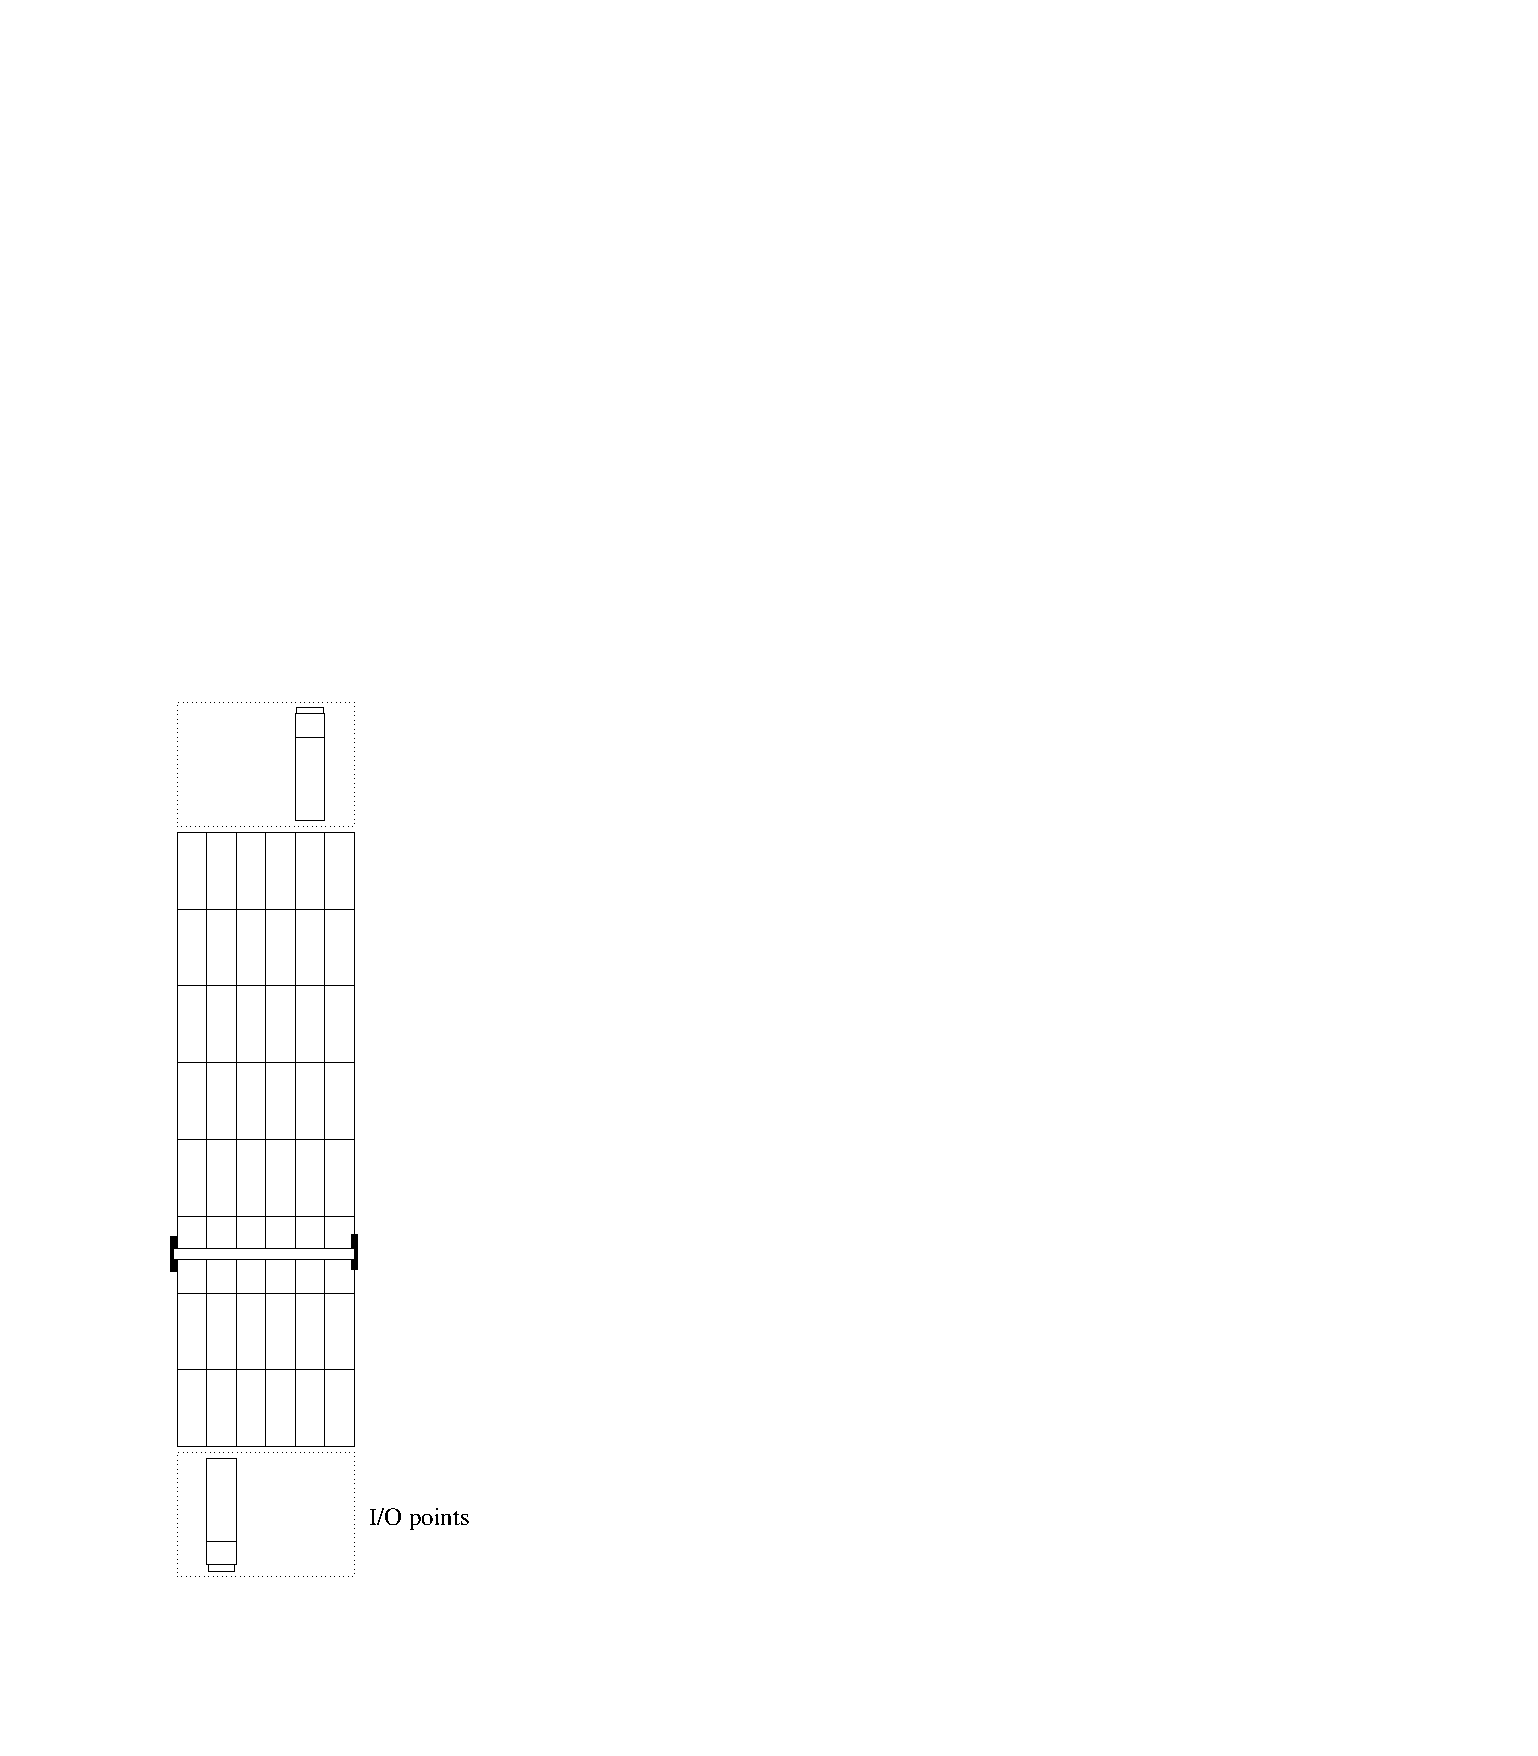
\includegraphics{fig15_2.pdf}}}
\caption{Two I/O layouts}
\label{fig15}
\end{figure}

Existing algorithms for the CPMP have not taken dummy stacks into consideration; hence, they cannot be implemented directly at terminal layouts as shown in Figure \ref{fig15:1}.
However, aforesaid terminal layouts are popular across the world.
This disparity between research and industrial practice must be resolved.

Our paper contributes to the literature in three aspects.
First, the CPMP is reexamined, and a new variant the CPMPDS, is proposed.
Second, a new lower bound suitable for both problems is proposed.
The new lower bound dominates the existing lower bounds with respect to the CPMP.
Last, three algorithms based on the idea of target-guided strategy are designed to solve both problems.
The algorithms fix containers at appropriately chosen positions and avoid further movements afterwards.
This mechanism reduces the problem size continuously until the problem is solved.
Thus, our algorithms guarantee termination.
Experimental results demonstrate that the proposed algorithms are better than the state-of-the-art algorithm to the best of our knowledge.
Although the CPMP is discussed in the context of maritime terminals, it is also applicable to other scenarios, such as warehouses and railway yards.

The remainder of this paper is structured as follows.
Section \ref{sec:litreview} presents an overview of existing works related to the CPMP.
Section \ref{sec:pd} formally defines the CPMP and CPMPDS.
Section \ref{sec:cf} discusses how to calculate lower bounds.
A greedy algorithm and two advanced beam search algorithms are elaborated in Section \ref{sec:heu} and Section \ref{sec:g2la}, respectively.
Section \ref{sec:ce} describes the experiments that were conducted to evaluate the effectiveness of the proposed algorithms and reports the results.
Finally, Section \ref{sec:con} concludes the research.

\section{Literature review}
\label{sec:litreview}

In recent years, publications in press concerning terminal operations, especially container handling, have exploded.
\cite{Vis2003} first provided an overview of the complex operations at container terminals and associated research problems.
\cite{Steenken2004} then provided an extensive description on main logistic processes and operations at container terminals, with a corresponding survey of optimization models and methods.
\cite{Stahlbock2008} presented new updates on container terminals.
In 2014, \cite{Carlo2014} provided a new in-depth overview of storage yard operations and highlighted current industrial development trends as well as associated future research directions.
Collectively, these studies point out that the CPMP is an important topic and worthy of more research effort.

Most existing methods for the CPMP are heuristic approaches.
\cite{Caserta2009} provided a greedy heuristic based on the paradigm of corridor and roulette wheel.
The corridor reduces movement choices for a certain layout and the roulette wheel provides randomness when making choices.
The probability of selecting an alternative is proportional to its attractiveness.
The algorithm first builds a corridor with respect to the current layout to determine the destination stacks of a specific misplaced container.
New layouts are then yielded by conducting the movements in the corridor.
The attractiveness of each new layout is evaluated by an estimated number of needed relocations.
A local improvement scheme is also conducted to accelerate the search process.
\cite{Exposito2012} proposed a multi-start heuristic to minimize the number of rehandles.
Movements were selected by a rule called ``low priority first''.
Thus, their method is more target-oriented than that of \cite{Caserta2009}.
In \cite{Exposito2012}, the concepts of corridor and roulette wheel were also used in building solutions.
A method was also given to generate instances and measure the difficulty of instances.

Unlike the above-mentioned approaches that construct solutions by finding promising movements step by step, a neighborhood search deployed by \cite{Lee2009} regards complete solutions as search units.
The neighborhood search obtains a new feasible solution by randomly modifying the current solution.
Solutions are shortened without disturbing solution feasibility by using a four-step procedure.
Three minor routines were also devised to diversify the resultant solutions and reduce the number of movements.
As it is very likely to generate infeasible solutions by random modifications, their method needs a large number of iterations.
Hence, the method is not as efficient as the heuristic of \cite{Exposito2012}.
\cite{Huang2012heu} solved two variants of the CPMP by a heuristic algorithm.
One variant allows containers of different groups to mix within a bay which is commonly seen.
The other variant is newly proposed which requires containers of different groups be separately located in the final layout.

Apart from heuristics, \cite{Lee2007} developed an IP model to tackle the CPMP.
They converted the CPMP into a multi-commodity network flow problem.
A network is composed of several subnetworks.
Each subnetwork represents an interim layout.
The nodes in a subnetwork correspond to slots of the bay, and containers are expressed as commodities.
A solution is expressed by a flow in the network.
The disadvantage of the algorithm is that the scale of networks is large even for small instances.
However, the algorithm provided an innovative view to investigate the CPMP.
\cite{BF2012} thoroughly described a tree search procedure and a new lower bound for the CPMP.
In the search tree, solutions are constructed by compound moves (several movements) instead of single movements, and branches are classified by four movement types.
The performance of the tree search is currently the best among all the extant methods.

As discussed by \cite{Caserta2011}, the counterparts of the CPMP include the container re-marshalling problem (CRMP) and the container relocation problem (CRP).
The CRMP refers to reassigning containers scattered within a block into their designated bays.
The CRMP is not a simple extension of the CPMP, because it involves multiple cranes.
The interference between multiple cranes and stacking positions of containers within a bay are the difficulties of the CRMP.
\cite{Caserta2011} proved that the CRMP is NP-hard.
\cite{Kim1998, Kang2006Plan, Park2009Plan, Choe2011} have exploited the CRMP and proposed some heuristic methods to cope with it.
The CRP aims to retrieve containers in a predetermined order with the fewest movements.
It had been studied by researchers by using various methods, ranging from meta-heuristics to simple heuristic algorithms \citep{Kim2006A, Yang2006A, Caserta2009A,Caserta2009Applying,Lee2010A,Caserta2012AM, Forster2012A, Zhu2012Iter,Jin2015}.


\section{Problem description}
\label{sec:pd}

The CPMP can be described as follows: Given a bay with $S$ stacks, each stack is able to store up to $H$ containers vertically.
Tiers of the bay are indexed from 1 to $H$ from the bottom up.
For consistency, the ground is considered as tier 0 in particular.
$N$ ($N\le S\times H$) containers are stored in the bay, which forms an initial layout with a usage rate of $N/(S\times H)$.
Each container $c$ is assigned a group label $g(c)\in \{1,\dots,G\}$.
The group labels of containers could be unique or duplicate.
Figure \ref{fig3} shows a layout with $S=5$, $H=6$, $G=9$, and duplicate group labels .

\begin{figure}[!htb]
\centering
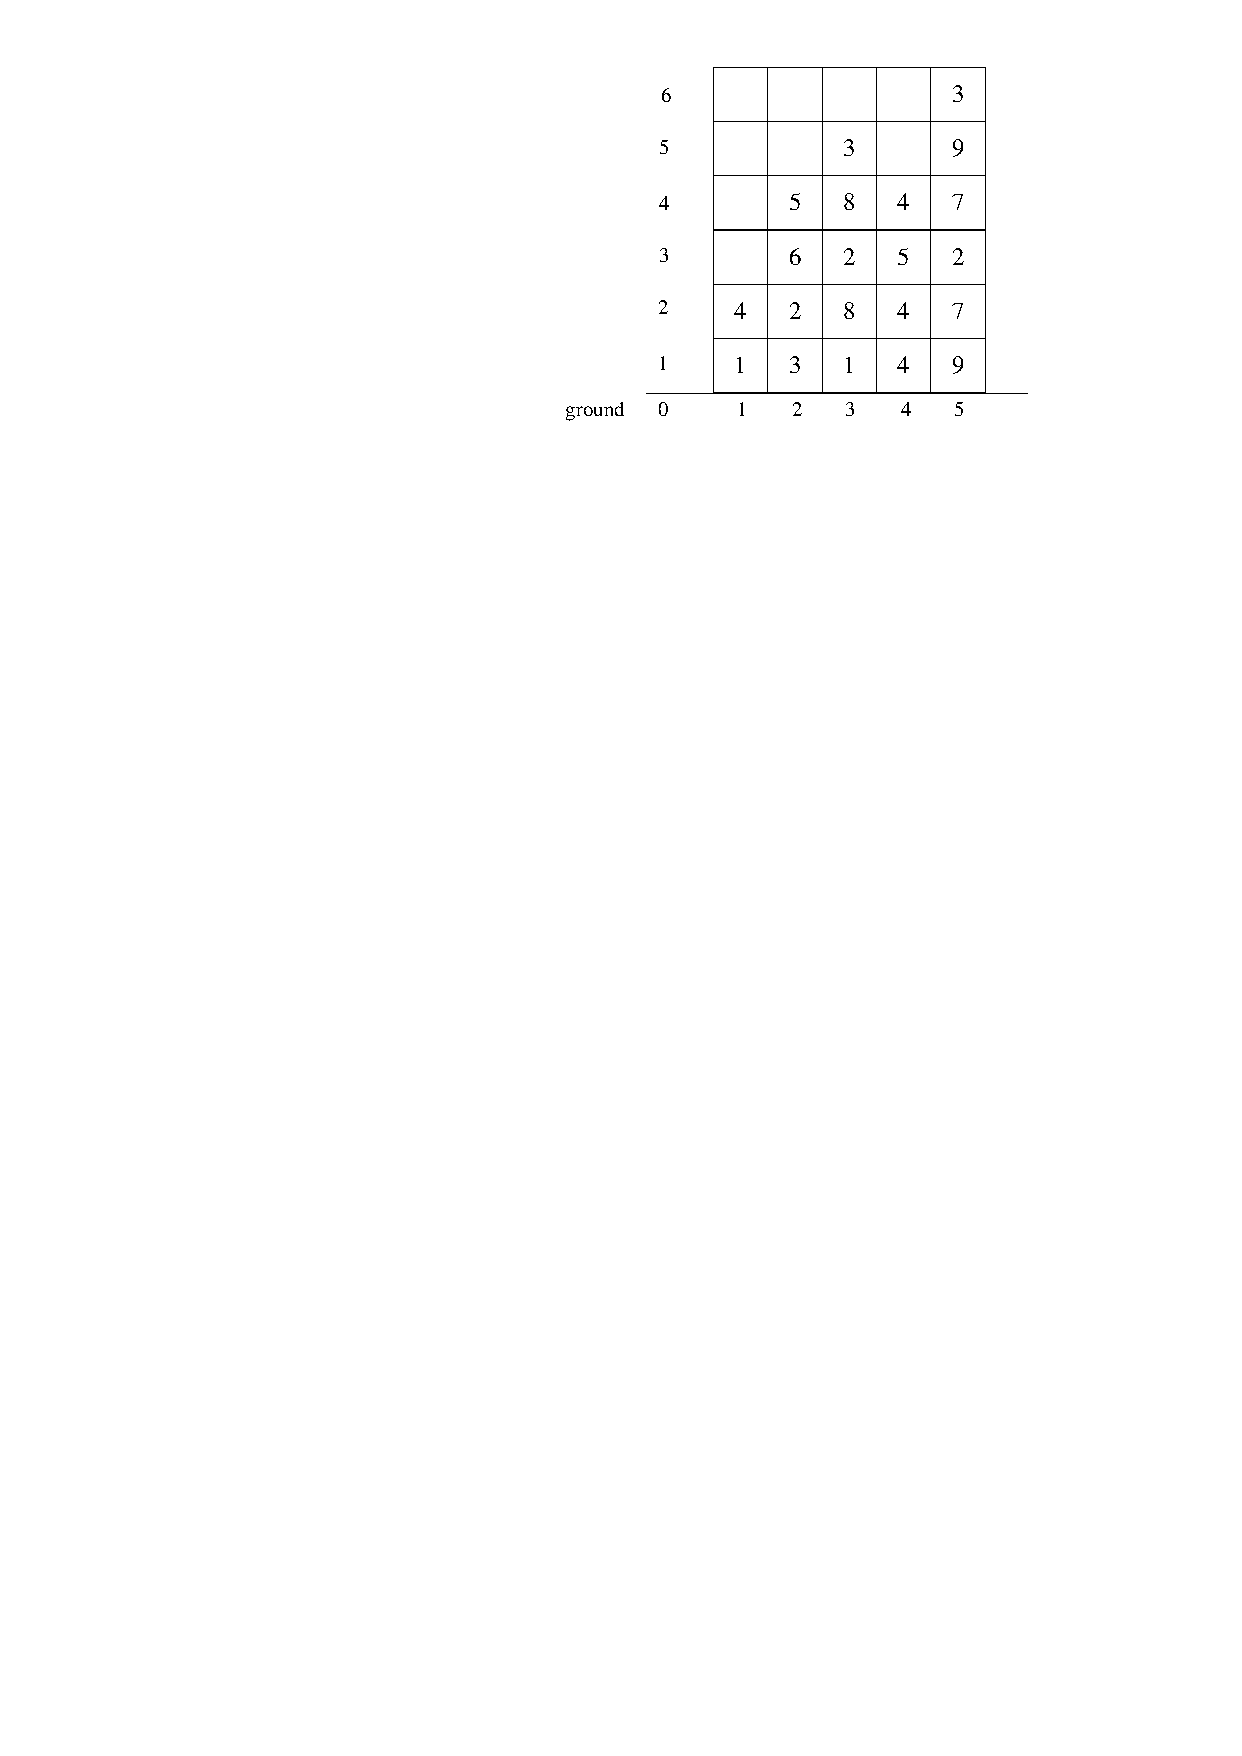
\includegraphics[width=0.35\textwidth]{fig3.pdf}
\caption{An example of a layout}
\label{fig3}
\end{figure}

One container can be moved from the top of a stack (\textbf{origin}) to the top of another stack (\textbf{destination}) if the destination stack is not fully occupied.
The CPMP is to find the shortest movement sequence that transforms the initial layout to a final layout with all stacks \textbf{clean}.
A stack is \textbf{clean} if its containers are piled in a non-increasing order of group labels from bottom to top; otherwise, the stack is \textbf{dirty}.
A stack $s$ can \textbf{accommodate} a container $c$ if and only if stack $s$ is clean and is still clean after $c$ is moved to its top.
A container $c$ is a clean container if and only if all the containers underneath are clean and their group labels are no smaller than $g(c)$; otherwise, $c$ is dirty.


In the new variant the CPMPDS, containers are only piled in the first $S-1$ stacks, and the $S$-th stack (i.e., the dummy stack) is empty in the initial layout.
The objective of CPMPDS is to transform the initial layout to a clean layout with an empty dummy stack by the least movement effort.
During pre-marshalling, containers can be placed in the dummy stack.
The dummy stack is always treated as a dirty stack, whatever containers are piled in it.
Analogously, containers in the dummy stack are regarded as dirty containers.
The dummy stack cannot accommodate any containers.

For ease of illustration, the notation used in this paper is defined in Table \ref{tab:1}.

\begin{table}[!htb]
  \centering
  \caption{Notation}
  \label{tab:1}
    \begin{tabular}{l|l}
    \hline
    Notations         & Description \\
    \hline
    $H$               &  height limitation of a bay\\
    $e(s)$            &  number of empty slots of stack $s$\\
    $h(s)$            &  number of containers of stack $s$\\
    $d(s)$            &  number of dirty containers of stack $s$\\
    $\mathit{uf}(s)$      &  number of unfixed containers of stack $s$\\
    $\mathit{sn}(c)$      &  stack where container $c$ is placed\\
    $\mathit{tn}(c)$      &  tier where container $c$ is placed\\
    $g(c)$            &  group label of container $c$\\
    $o(c)$          &  number of containers above container $c$\\
    \hline
    \end{tabular}
\end{table}

\section{Lower bound}
\label{sec:cf}

In this section, a new method is proposed to calculate the lower bound of the number of necessary movements to reach a clean layout.
The calculation of the lower bound for the CPMP is demonstrated first.
The lower bound for the CPMPDS only requires a slight modification on that for the CPMP.

\subsection{Lower bound for the CPMP}

The lower bound is obtained by estimating the number of movements that belong to different movement types.

\begin{enumerate}
\setcounter{enumi}{0}
\item Dirty--Clean movements
\end{enumerate}

The number of dirty containers in a given layout is $\sum_{s=1}^S d(s)$.
Each dirty container requires at least one movement to become clean; thus, the lower bound of the number of Dirty--Clean movements is $\mathit{num}_\mathit{DC}=\sum_{s=1}^S d(s)$.

\begin{enumerate}
\setcounter{enumi}{1}
\item Dirty--Dirty movements
\end{enumerate}

If all the stacks are dirty in a layout, at least one stack should become clean first, in order to create possibility to accommodate containers.
This purpose is realized by moving dirty containers of a stack to other dirty stacks.
The least number of Dirty--Dirty movements for making a stack clean is $\mathit{num}_\mathit{DD} = \min_s d(s)$.

\begin{enumerate}
\setcounter{enumi}{2}
\item Clean--X movements
\end{enumerate}

Before proceeding to explain the calculation of Clean--X movements, the concept of skyline should be introduced first.
A skyline is any vertical partition that separates a layout into higher and lower parts, where the lower part must be clean.
A skyline can be represented by a vector $\mathit{SL}$ such that each element $\mathit{SL}_s$ represents the skyline segment across stack $s$.
The tier and group numbers of $\mathit{SL}_s$ are equal to those of the container underneath.
For example, in Figure \ref{fig5}, the bold line presents a skyline of the layout with $\mathit{tn}(\mathit{SL}_{2})=3$ and $g(\mathit{SL}_{2})=1$.


\begin{figure}[!htb]
\centering
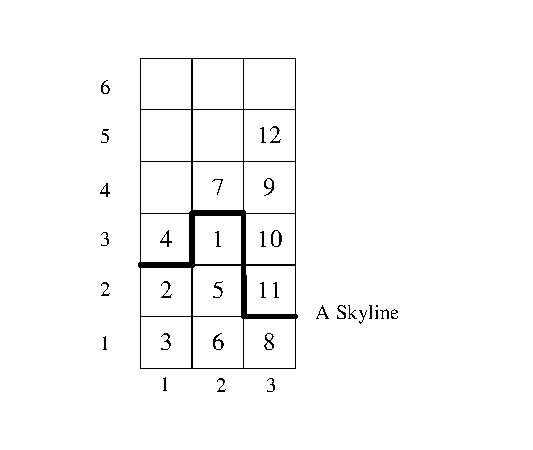
\includegraphics[width=0.25\textwidth]{fig5.pdf}
\caption{A skyline of a layout}
\label{fig5}
\end{figure}

Supply and demand vectors, denoted by $\mathbf S^\mathit{SL}$ and $\mathbf D^\mathit{SL}$, record the numbers of slots and containers above $\mathit{SL}$.
The $g$-th element of $\mathbf S^\mathit{SL}$ is
\[
\mathbf S^\mathit{SL}_g=\sum_{s:g(\mathit{SL}_s)=g}H-\mathit{tn}(\mathit{SL}_s)\textrm{,}
\]
whereas the $g$-th element of $\mathbf D^\mathit{SL}$ is the number of containers with group labels $g$ above $\mathit{SL}$.

For ease of explanation, Clean--Dirty and Clean--Clean movements are merged as Clean--X movements.
The number of moved clean containers is a lower bound of the number of Clean--X movements.
Ideally, pre-marshalling work involves dirty containers only and leaves clean containers unmoved.
In some cases, however, achieving a clean layout is impossible if keeping all the clean containers unmoved.
The number of clean containers that need to be moved can be counted by the following process: given a bay, all the dirty containers and a set of clean containers $C$ are removed from the layout, then slots are reassigned to removed containers.
The resultant layout is required to be clean.
Removed containers within a stack should be consecutive, i.e., if two containers from the same stack are removed, containers between them are also removed.
The size of the smallest $C$ is the lower bound of the number of required Clean--X movements ($\mathit{num}_{CX}$).
Finding the smallest $C$ is equivalent to finding the skyline with the fewest clean containers in its higher part (smallest skyline), such that the differences of the supply and demand vectors (surpluses) for all groups are non-negative (see Equation \ref{equ:3}).

\begin{equation}
\label{equ:3}
\sum_{i\ge g}\mathbf S^\mathit{SL}_i-\sum_{i\ge g}\mathbf D^\mathit{SL}_i\ge0, \quad g=1,\dots,G\textrm{.}
\end{equation}

To find the smallest skyline, a basic skyline $\mathit{SL}$ that separates clean and dirty containers is drawn.
Next, a depth-first-search (DFS) is deployed to push a certain segment of $\mathit{SL}$ one tier down in each branch.
The leaves of the search tree are all the skylines with non-negative surpluses; the one with the fewest pushes is selected and the number of pushes is $\mathit{num}_\mathit{CX}$.

To conclude, the lower bound is finally yielded as $\mathit{LB}_\mathit{DFS}=\mathit{num}_\mathit{DC}+\mathit{num}_\mathit{DD}+\mathit{num}_\mathit{CX}$.

\subsection{Computing Clean--X movements by maximum knapsack}

The lower bound $\mathit{LB}_\mathit{DFS}$ is time consuming because a DFS is used to calculate $\mathit{num}_{\mathit{CX}}$.
A maximum knapsack method (MKM) is proposed to approximate $\mathit{num}_{CX}$.
A basic skyline $\mathit{SL}$ that separates clean and dirty containers is drawn, then the smallest skyline with non-negative surplus for a single group instead of all groups is obtained.
This search is repeated for each group, and the largest number of pushes is selected amongst all groups.

For a given group label $g$, a knapsack problem is solved to find the smallest skyline with non-negative surplus in terms of $g$.
Stacks in the bay are regarded as items, where each item $s\in\{1,\dots,S\}$ has value $v_s$ and cost $c_s$.
The objective is to select a set of items with the lowest cost such that the total value selected is at least $V$.
Every item can only be selected at most once.
$c_s$ is the number of clean containers in stack $s$ to be moved to accommodate group $g$, while $v_s$ is the resultant number of slots available for group $g$, i.e., $v_s=c_s+e(s)$.
$V$ is the number of dirty containers with group labels $g(c)\ge g$.
The decision variable $x_s$ is 1 if stack $s$ is selected; otherwise, $x_s=0$.
The integer programming model of this knapsack problem is given in Equation \ref{equ:4} and can be solved easily by dynamic programming.

\begin{equation}
\label{equ:4}
\begin{array}{rl}
\min & \sum_{s=1}^S c_s x_s\\
\mathrm{s.t.} &\sum_{s=1}^S v_s x_s\ge V\\
&x_s\in\{0,1\}, \quad s=1,\dots,S\textrm{.}
\end{array}
\end{equation}

MKM is not as precise as DFS, but the solution gap is quite small and the computation speed is improved.
The lower bound provided by MKM is denoted by $\mathit{LB}_{\mathit{MKM}}$.

\subsection{Comparison with existing lower bound}

The current state-of-the-art lower bound $\mathit{LB}_\mathit{BF}$ is proposed by \cite{BF2012} which also consists of three parts: Dirty--Clean, Dirty--Dirty and Clean--X movements.
The first two types are calculated in the same way as $\mathit{LB}_\mathit{DFS}$ and $\mathit{LB}_\mathit{MKM}$ in this paper. The calculation of Clean--X movements is different.
A basic skyline $\mathit{SL}$ that separates clean and dirty containers is drawn, then \cite{BF2012} only take the group label $g^*$ with the smallest surplus $g^*=\arg\min_g\sum_{i\ge g}\mathbf S^\mathit{SL}_i-\sum_{i\ge g}\mathbf D^\mathit{SL}_i$.

If $\mathit{min}=\sum_{i\ge g^*}\mathbf D^\mathit{SL}_i-\sum_{i\ge g^*}\mathbf S^\mathit{SL}_i$ is negative, it means that clean containers need to be moved to accommodate $|\mathit{min}|$ dirty containers.
The number of moved clean containers $\mathit{num}_\mathit{CX}$ is estimated by \cite{BF2012} as follows: suppose one stack is able to (as a matter of fact, it may not be able to) accommodate $H$ dirty containers with $g\ge g^*$, then $|\mathit{min}|$ dirty containers need at least $\big\lceil{|\mathit{min}|}/{H}\big\rceil$ stacks.
As slots supply of stacks with $g(\mathit{SL}_s)\ge g^*$ have been calculated into $\sum_{i\ge g^*}\mathbf S^\mathit{SL}_i$, only stacks with $g(\mathit{SL}_s)< g^*$ can supply slots for $|\mathit{min}|$ dirty containers.
From such stacks, the first $\big\lceil{|\mathit{min}|}/{H}\big\rceil$ stacks (denoted by set $\mathit{AS}$) with the smallest values of $c_s$ are selected, where $c_s$ is the number of clean containers in a stack $s$ to be moved to accommodate group $g^*$.
Finally, $\mathit{num}_\mathit{CX}=\sum_{s\in \mathit{AS}}c_s$.

From the mathematical perspective, the method of \cite{BF2012} is equivalent to solving the following model: stacks in the bay are regarded as items, where each item $s\in\{1,\dots,S\}$ has value $v_s'$ and cost $c_s$.
The objective is to select a set of items with the lowest cost such that the total value selected is at least $V$.
Every item can only be selected at most once.
$c_s$ is the number of clean containers in stack $s$ to be moved to accommodate group $g^*$, while $v_s'$ is the resultant number of slots available for group $g^*$.
According to \cite{BF2012}, $v_s'=H$ if $g(\mathit{SL}_s)<g^*$; otherwise, $v_s'=c_s+e(s)$.
$V$ is the number of dirty containers with group labels $g(c)\ge g^*$.
The decision variable $x_s$ is 1 if stack $s$ is selected; otherwise, $x_s=0$.
The integer programming model is shown in Equation \ref{equ:5}.

\begin{equation}
\label{equ:5}
\begin{array}{rl}
\min & \sum_{s=1}^S c_s x_s\\
\mathrm{s.t.} &\sum_{s=1}^S v_s' x_s\ge V\\
&x_s\in\{0,1\}, \quad s=1,\dots,S\textrm{.}
\end{array}
\end{equation}

Comparing Model \ref{equ:4} with Model \ref{equ:5}, all the parameters are the same except $v_s$ and $v_s'$.
Since $v_s\le v_s'$ for any $s$, any feasible solution to Model \ref{equ:5} is a feasible solution to Model \ref{equ:4}, while the reverse does not stand.
The solution space of Model \ref{equ:5} is a superset of that of Model \ref{equ:4}, thus the optimal solution to Model \ref{equ:4} is no smaller than that to Model \ref{equ:5}.
Furthermore, \cite{BF2012} only solve Model \ref{equ:5} once for $g^*$, whereas this paper solves Model \ref{equ:4} for every group and then takes the maximum objective value as $\mathit{num}_\mathit{CX}$.
As a result, the lower bound $\mathit{LB}_\mathit{MKM}$ dominates $\mathit{LB}_\mathit{BF}$: $\mathit{LB}_\mathit{BF}\le \mathit{LB}_\mathit{MKM}\le \mathit{LB}_\mathit{DFS}$.

\subsection{Lower bound for the CPMPDS}


The lower bound for the CPMPDS also consists of three parts: Dirty--Clean, Dirty--Dirty, and Clean--X movements.

The lower bound of Dirty--Clean movements is equal to the number of dirty containers.
For Dirty--Dirty movements, $\mathit{num}_\mathit{DD}=\min_{s\neq s_d} d(s)$, where $s_d$ is the dummy stack.
If all the ordinary stacks are dirty, then dirty containers from at least one ordinary stack need to be relocated to other dirty ordinary stacks or the dummy stack.
In both situations, these relocated containers are still dirty after relocation.

The lower bound of Clean--X movements is the number of clean containers that need to be moved, so as to make all the containers clean and the dummy stack empty, which is equivalent to assigning containers only to the ordinary stacks and ignoring the dummy stack.

Based on the analysis above, $\mathit{LB}_\mathit{DFS}$ ($\mathit{LB}_\mathit{MKM}$) for a CPMPDS instance is equal to that for the corresponding CPMP instance with the dummy stack removed.

\section{Target-guided heuristic}
\label{sec:heu}

This section presents a target-guided heuristic (TGH) for the CPMP/CPMPDS.
This heuristic can be used as an independent algorithm as well as a component of more complex algorithms in the next section.

The main idea of the heuristic is to fix containers to certain stacks in a descending order of their group labels.
Among all unfixed containers in the incumbent layout, containers with the largest group label are called \textbf{candidate containers}.
At each step, a candidate container and a candidate stack are selected as a target pair.
By a sequence of movements, the target container is finally moved to the lowest unfixed slot of the target stack.
After that, the target container is fixed and avoids further movement.
Only one special situation is able to relocate a fixed container, but the relocated fixed container will be moved back to its fixed position later; this action will be explained later.

As containers are fixed sequentially, all the stacks become clean in the end.
Hence, this heuristic guarantees a feasible solution for any solvable instance.
A complete description of the framework is shown in Algorithm \ref{alg:heu}.

\begin{algorithm*}[!htb]
	\caption{The target-guided heuristic for the CPMP/CPMPDS}
	\label{alg:heu}
	\begin{codebox}
	\Procname{\proc{TGH ($\mathit{inilay}$)}}
	\li $\mathit{curlay} = \mathit{inilay}$
    \li $\mathit{g} = G$
    \li \While $g\neq0$
    \li \Do
            mark clean containers with group labels $g$ as fixed\label{heu:c}
    \li     $\mathit{conList} = $ the set of candidate containers
    \li     \While $\mathit{conList} \neq \varnothing$\label{heu:l}
    \li     \Do
                $\mathit{stkList} = $ the set of candidate stacks
    \li         determine the target container and stack from $\mathit{conList}$ and $\mathit{stkList}$, respectively
    \li         apply a giant move to fix the target container to the target stack
            \End
    \li $g=g-1$
        \End
	\end{codebox}
\end{algorithm*}


The advantage of the proposed heuristic is that containers are fixed one by one.
Therefore, customizing the heuristic for other CPMP variants, such as variants that require containers in a final layout adhere to special distribution characteristics, is easy.
The heuristic only needs to modify candidate stack selection rules according to the required distribution.

\subsection{Candidate container and stack selection}
\label{sec:can}

The set of candidate containers when processing group $g$ comprises all unfixed containers with group labels $g$.
A set of candidate stacks are selected based on the set of candidate containers and each candidate stack $s$ must satisfy $\id{uf}(s)\le\sum_{i\neq s}e(i)$ and be able to accommodate group $g$ after relocating its unfixed containers.
If there exists no such a stack, then the instance is unsolvable.
If there exist multiple such stacks, those stacks that can accommodate $g$ without any relocation is preferred; otherwise, other stacks are selected.

\subsection{Target pair selection}
\label{sec:tar}

An evaluation scheme is designed to evaluate the attractiveness of fixing a candidate container to a candidate stack.
Intuitively, fewer movements for fixing is preferred.
A function $f(c,s)$ is introduced to roughly estimate the movement cost for fixing container $c$ to stack $s$.
If $c$ is currently in $s$, $f(c,s)=\mathit{uf}(s)$; otherwise, $f(c,s)=\mathit{uf}(s)+o(c)$.
Stacks with smaller numbers of fixed containers $h(s)-\mathit{uf}(s)$ are preferred.
This preference distributes fixed containers evenly among stacks.
Thus, two-tuple $(f(c,s), h(s)-\mathit{uf}(s))$ evaluates the attractiveness.

Each candidate container and each candidate stack make up a candidate pair.
All the candidate pairs are sorted in an ascending lexicographical order of evaluation values, and the best one is selected as the target pair.

\subsection{Giant move}

Given target container $c^*$ and target stack $s^*$, a giant move is executed to fix $c^*$ in $s^*$.
The target slot in $s^*$ for $c^*$ is the slot just above fixed containers of $s^*$.
Hereafter, the target slot will not be explicitly pointed out, because a giant move does not disturb positions of fixed containers.
According to whether the origin of $c^*$ is $s^*$ or not, the giant move includes two cases.

\subsubsection{Case 1: Fixing to the same stack}

In Case 1, the origin of $c^*$ is $s^*$.
In the first step, all the containers above $c^*$ are relocated; the relocation strategy will be explained in Section \ref{sec:rel}.
After that, $c^*$ is at the top of $s^*$ and needs a stack for temporary storage.
The highest non-full stacks are considered for temporary storage; among such stacks, a dirty stack is preferred. The selected temporary stack is denoted by $\mathit{ts}$.

Before moving $c^*$ to $\mathit{ts}$, observe in advance the relocation positions of unfixed containers under $c^*$ so that $s^*$ can accommodate $c^*$.
Avoiding occupying both $\mathit{ts}$ and $s^*$ is a straightforward idea.
On top of this, denote the set of stacks except $\mathit{ts}$ and $s^*$ by $\mathit{AS}$, compute its available empty slots $\mathit{nslot} = \sum_{s\in \mathit{AS}}e(s)$, and compare $\mathit{nslot}$ with $\mathit{uf}(s^*)$.
According to comparison results, three scenarios are raised.

\begin{enumerate}
\setcounter{enumi}{0}
\item $\mathit{nslot}\ge \mathit{uf}(s^*)-1$
\end{enumerate}

In this scenario, the empty slots of $\mathit{AS}$ are enough to store unfixed containers under $c^*$. $c^*$ is moved directly to $\mathit{ts}$, then all the unfixed containers of $s^*$ are relocated to empty slots of $\mathit{AS}$.
Finally, $c^*$ is moved back to $s^*$.

\begin{enumerate}
\setcounter{enumi}{1}
\item $0<\mathit{nslot}< \mathit{uf}(s^*)-1$
\end{enumerate}

In this scenario, the empty slots of $\mathit{AS}$ are not enough for unfixed containers under $c^*$. After moving $c^*$ to $\mathit{ts}$, only the first $\mathit{nslot}-1$ unfixed containers are relocated to the empty slots of $\mathit{AS}$, leaving one empty slot.
The last empty slot is occupied by moving $c^*$ to it from $\mathit{ts}$.
The remaining unfixed containers in $s^*$ are then relocated to $\mathit{ts}$.
At last, $c^*$ is moved back to $s^*$.

\begin{enumerate}
\setcounter{enumi}{2}
\item $\mathit{nslot}=0$
\end{enumerate}

In this scenario, all the stacks in $\mathit{AS}$ are full.
$c^*$ cannot be moved directly to $\mathit{ts}$; otherwise, it will be buried by unfixed containers in $s^*$.
A top slot is needed to temporarily store $c^*$.
To create such an empty slot, a top container $c$ is found from all the top containers of stacks in $\mathit{AS}$.

If $\mathit{ts}$ is a clean stack, the preference is as follows:
\begin{enumerate}[1.]
\item Among dirty containers that $\mathit{ts}$ can accommodate, the one with the largest group label is selected;
\item Among clean containers that $\mathit{ts}$ can accommodate, the one with the largest group label is selected;
\item The dirty container with the smallest group label is selected;
\item The clean container with the smallest group label is selected.
\end{enumerate}

If $\mathit{ts}$ is a dirty stack, the preference is:
\begin{enumerate}[1.]
\item The dirty container with the smallest group label is selected;
\item The clean container with the smallest group label is selected.
\end{enumerate}

After $c$ is moved to $\mathit{ts}$, its origin is occupied by $c^*$.
All the unfixed containers of $s^*$ are relocated to $\mathit{ts}$.
Finally, $c^*$ is moved to $s^*$.

The special situation mentioned above Algorithm \ref{alg:heu} arises if $c$ is a fixed container, where $c$ should be restored to its originally fixed slot.
Suppose the origin of $c$ is stack $\mathit{cs}$, all the containers above $c$ are relocated and $c$ is moved back to $\mathit{cs}$.

\subsubsection{Case 2: Fixing to a different stack}

In Case 2, the origin of $c^*$ is not $s^*$.
If $c^*$ is the topmost container and all the containers in $s^*$ are fixed, $c^*$ is moved to $s^*$ directly.
Otherwise, in spirit of Case 1, $\mathit{AS}$ is defined as the set of all the stacks except $s^*$ and $\mathit{sn}(c^*)$ (the origin of $c^*$) and the fewest required movements $f(c^*,s^*)$ are compared with the number of available slots $\mathit{nslot}=\sum_{s\in \mathit{AS}}e(s)$.
According to comparison results, four scenarios are raised.

\begin{enumerate}
\setcounter{enumi}{0}
\item $\mathit{nslot}\ge f(c^*,s^*)$
\end{enumerate}

In this scenario, all the containers above $c^*$ and unfixed containers in $s^*$ are relocated to empty slots of $\mathit{AS}$. The top container from $s^*$ or $\mathit{sn}(c^*)$ is relocated at a time, whichever has a larger group label. After that, $c^*$ is moved to $s^*$.

\begin{enumerate}
\setcounter{enumi}{1}
\item $o(c^*)+1\le\mathit{nslot}< f(c^*,s^*)$
\end{enumerate}

In this scenario, containers above $c^*$ and unfixed containers in $s^*$ cannot be relocated to empty slots of $\mathit{AS}$ one-off.
A total of $\mathit{nslot}-1$ containers, including all the containers above $c^*$ together with a subset of unfixed containers in $s^*$ are relocated, which leaves one empty slot for $c^*$.
The topmost container with a larger group label is relocated at a time.
After relocating aforesaid containers, $c^*$ is moved to the unique empty slot left in $\mathit{AS}$, after which all the remaining unfixed containers in $s^*$ are relocated to $\mathit{sn}(c^*)$.
At last, $c^*$ is moved to $s^*$.

\begin{enumerate}
\setcounter{enumi}{2}
\item $1\le\mathit{nslot}< o(c^*)+1$
\end{enumerate}

In this scenario, $\mathit{nslot}-1$ containers of $\mathit{sn}(c^*)$ are relocated to empty slots of $\mathit{AS}$; the remaining containers above $c^*$ are then relocated to $s^*$.
$c^*$ is currently on top and moved to the unique empty slot in $\mathit{AS}$.
All the unfixed containers in $s^*$, including those originated from $\mathit{sn}(c^*)$, are relocated to $\mathit{sn}(c^*)$.
At last, $c^*$ is moved to $s^*$.

\begin{enumerate}
\setcounter{enumi}{3}
\item $\mathit{nslot}=0$
\end{enumerate}

This scenario is similar to Scenario 3 of Case 1, where $c^*$ needs an empty slot for temporary storage.
The selection of a top container from a full stack is the same as the process in Scenario 3 of Case 1.
The selected top container is denoted as container $c$ and its origin as stack $\mathit{cs}$.
$c$ is first moved to $s^*$, then all the containers above $c^*$ are relocated to $s^*$.
$c^*$ is moved to $\mathit{cs}$ for temporary storage.
Next, all the unfixed containers of $s^*$ ($c$ included) are relocated to $\mathit{sn}(c^*)$.
At last, $c^*$ is moved to $s^*$.
Similar to the issue raised in Scenario 3 of Case 1, $c$ may be a fixed container.
If that is the case, $c$ also has to be restored to $\mathit{cs}$.


\subsection{Container relocation}
\label{sec:rel}

Container relocation occurs when a container blocks the target container or if it is an unfixed container in the target stack.
Generally speaking, a container $c$ can be relocated to any stack, excluding prohibited stacks such as the target stacks, origins of target containers, and sometimes temporary stacks for target containers.
Preferably, $c$ should be relocated to an appropriate stack so that it will not block or be blocked by other containers in the future.
Suppose the target container in the process is $c^*$.
Apart from prohibited and full stacks, the destination stack for relocating $c$ is found based on the following preference.

\begin{enumerate}[1.]
\item A clean stack that can accommodate $c$ is selected. If several such stacks exist, the one with the top container that has the smallest group label is selected;

\item A dirty stack in which the largest group label of dirty containers $\mathit{ldg}$ is no larger than $g(c)$ is selected. If several such stacks exist, the one with the largest $\mathit{ldg}$ is selected;

\item A dirty stack in which the largest group label of dirty containers $\mathit{ldg}$ satisfies $g(c)<\mathit{ldg}<g(c^*)$ is selected. If several such stacks exist, the one with the smallest $\mathit{ldg}$ is selected;

\item A clean stack with the top container that has the largest group label is selected;

\item A dirty stack in which the largest group label of dirty containers $\mathit{ldg}$ is equal to $g(c^*)$ is selected.
\end{enumerate}


If the selected destination can accommodate container $c$, an extra action called \textbf{fulfillment} is carried out.
Denote the topmost container of the destination stack as $\mathit{dc}$.
If there exists a set of topmost dirty containers with group labels between $g(c)$ (exclusive) and $g(\mathit{dc})$ (inclusive), the one with the largest group label is selected and moved to the destination stack.

If fulfillment is carried out successfully, the relocation procedure for $c$ is re-invoked.
The advantage of fulfillment is that slots of clean stacks are utilized, which prevents containers with small group labels from occupying the top of a stack and blocking it from accommodating dirty containers with larger group labels.
Fulfillment is efficient at the start of the heuristic when a large number of dirty containers with large group labels are present.

In the proposed heuristic, only one movement is carried out each time the fulfillment is invoked, after which the heuristic turns to relocating containers.
This situation is different from that of \cite{Exposito2012} which carries out as many movements as possible in one fulfillment.
Performing one movement in one fulfillment is preferred because the aim is to relocate $c$, whereas fulfillment is only an auxiliary operation.
Compared with greedily conducting movement in one fulfillment, determining whether a more suitable stack for $c$ results from the fulfillment is more important.
Executing more movements in one fulfillment deviates from the aim of relocating $c$.
Moreover, over-fulfillment may cause stacks fulfilled to be emptied in later stages, which produces more movements.

\subsection{Termination analysis}

In Algorithm \ref{alg:heu}, the proposed heuristic fixes containers one by one and therefore guarantees a solution for any feasible instance. The fact that a fixed container may be moved when fixing another container was not mentioned.
If this situation occurs, the heuristic cannot be guaranteed to terminate because it may fall into cycling.
Fortunately, this issue is successfully resolved: a fixed container can only be moved when $\mathit{nslot}=0$.
In other situations, all the moved containers are unfixed ones. Once a fixed container is moved, it recovers to its fixed position (i.e., the last scenarios of Case 1 and 2).
Undoubtedly, this recovery action produces more movements; however, it avoids the heuristic cycling in vain and assures that the heuristic terminates with a feasible solution.
All other published works that concern the CPMP, except for this work, fail to guarantee algorithm termination and a feasible solution theoretically.

\section{Beam search algorithms}
\label{sec:g2la}

Algorithm \ref{alg:heu} is just a greedy heuristic, the core idea of which is to fix containers one by one, and selecting target containers and stacks is completely based on the evaluation scheme.
Obviously, the precision of the scheme is very important; once the scheme fails, the heuristic is led to a wrong direction.
To avoid this risk, beam search algorithms are proposed in this section, which can be applied to both the CPMP and the CPMPDS.

\subsection{Beam search with giant moves}

The first beam search algorithm maintains a beam of promising layouts and the number of such promising layouts in the beam is a user-defined parameter $\mathit{bw}$ (beam width).
Initially, the beam contains only the initial layout.
The layouts in the beam are extended iteratively by giant moves, hence the name -- beam search with giant moves (BS-G).

For each layout $l$ in the beam, a probing tree search is performed on $l$ with tree width $\mathit{tw}$ and tree depth $\mathit{td}$ to generate its children by selecting container-stack pairs and conducting corresponding giant moves.
Only a few of container-stack pairs are selected; pairs with container and stack parts in the candidate container and stack lists, respectively, are considered.
Candidate containers and stacks are produced in the same process as mentioned in Section \ref{sec:can}.
All candidate pairs are sorted based on the evaluation scheme values in Section \ref{sec:tar}.
The first $\mathit{tw}$ pairs are selected, and the corresponding giant moves are executed, which obtains $\mathit{tw}$ children of $l$.
$l$ is regarded as at depth 0; the tree expansion continues until depth $\mathit{td}$ is arrived with at most $\mathit{tw}^\mathit{td}$ layouts, which are called leaves of the tree, though they are not necessarily clean layouts.
Each leaf is further extended by invoking TGH in Section \ref{sec:heu} repeatedly to obtain a clean layout.
The scores of clean layouts are marked by the number of movements executed from the initial layout.
In the end, the score of a child of $l$ (layout at depth 1) is the best score among scores of clean offspring layouts.

Every layout in the beam generates at most $\mathit{tw}$ children based on a probing tree mentioned above, and there are at most $\mathit{bw}$ layouts in the beam.
Therefore, at most $\mathit{tw}\times \mathit{bw}$ children are generated.
They are sorted in a descending order of scores, and the first $\mathit{bw}$ children are selected into the beam for the next iteration.
The pseudo-code is shown in Algorithm \ref{alg:bsg}.

\begin{algorithm*}[htbp]
	\caption{Beam search with giant moves for the CPMP/CPMPDS}
	\label{alg:bsg}
	\begin{codebox}
	\Procname{\proc{BS-G ($\mathit{inilay}$)}}
    \li $\mathit{beam} = \{\mathit{inilay}\}$
    \li \While $\mathit{beam} \neq \varnothing$
    \li \Do
        $\mathit{canlaylist}=\varnothing$
    \li \For each $\mathit{lay}$ in $\mathit{beam}$
    \li     \Do
             generate up to $\mathit{tw}$ children of $\mathit{lay}$ and append the children to $\mathit{canlaylist}$
             \End
    \li     sort the layouts in $\mathit{canlaylist}$ in a descending order of scores
    \li     $\mathit{beam} =$ the first $\mathit{bw}$ layouts in $\mathit{canlaylist}$
        \End
	\end{codebox}	
\end{algorithm*}

\subsection{Beam search with baby moves}

In Algorithm \ref{alg:heu}, a movement sequence that fixes a target container to a target stack is named as a \textbf{giant move}.
By contract, a single-movement operation is coined as a \textbf{baby move}.

The successor generation method of BS-G is modified to obtain another algorithm for the CPMP and the CPMPDS.
In this algorithm, a beam search is deployed to maintain the diversity of layouts; the difference from BS-G is that successors in the beam are generated by applying baby moves, hence the name beam search with baby moves (BS-B).
BS-B does not have the disadvantage of BS-G that each giant move goes too far.
Apart from the successor generation method, other components in BS-B and BS-G are the same.
The process of generating successors in BS-B is as follows:

Probing tree search is applied to each layout $l$ in the beam as described in BS-G to generate $\mathit{tw}$ children.
The score of a child $\mathit{chi}$ is the minimum score of clean offspring layouts expanded from $\mathit{chi}$.
For each child $\mathit{chi}$ of $l$, the first interim layout on the path from $l$ to $\mathit{chi}$ is recorded, and the score of this interim layout that is the same as the score of $\mathit{chi}$, is marked.
If an interim layout is the first interim layout of multiple children, the smallest score is marked.
The successors of $l$ in BS-B are such interim layouts, instead of the children of $l$.

\subsection{Discussion on the CPMPDS}

In this paper, three interrelated algorithms are proposed: TGH, BS-G and BS-B.
These algorithms can be applied to solve the CPMP and the CPMPDS instances. Existing algorithms for the CPMP cannot be applied directly to solve the CPMPDS instances because they cannot guarantee that the dummy stack is empty after pre-marshalling.
If the dummy stack is ignored and a CPMPDS instance is attempted to be solved by using existing algorithms for the CPMP, feasible solutions may not exist because of the shortage of available empty slots.

\section{Experiments and analysis}
\label{sec:ce}

The proposed algorithms are tested against the benchmark test data sets provided by \cite{BF2012} to evaluate their effectiveness.
The performance of the proposed lower bounds and that of \cite{BF2012} is first compared. Then a series of experiments are conducted to evaluate the performance of the evaluation scheme and search parameters, which is followed by the results on benchmark data.
A data set for the new CPMPDS is generated, and the result is presented for further reference.
Experiments were conducted on a PC with Intel Core i7 CPU clocked at 3.40 GHz with Windows 7 operating system.

\subsection {Lower bound comparison}

Benchmark data are used to compare the performance of $\mathit{LB}_\mathit{DFS}$, $\mathit{LB}_\mathit{MKM}$, and $\mathit{LB}_\mathit{BF}$.
In Table \ref{tab:lowerbound}, columns DFS, MKM, and BF indicate average lower bounds of instances in corresponding data sets calculated by $\mathit{LB}_\mathit{DFS}$, $\mathit{LB}_\mathit{MKM}$ and $\mathit{LB}_\mathit{BF}$, receptively.
As such, columns tDFS, tMKM and tBF are the average computational time of the three methods in seconds which can be regarded as no difference.
Table \ref{tab:lowerbound} shows that DFS and MKM have better performance than BF, but the improvement is tiny.

\begin{table}[!htb]
\centering
\caption{\label{tab:lowerbound} Lower bound comparison}
\begin{tabular}{c|c|c|c|c|c|c}
    \hline
    data &    DFS     &     MKM   &   BF     & tDFS    & tMKM   & tBF \\
    \hline
    LC       &   29.780   &   29.659  &  29.659  & $<1$    & $<1$   & $<1$ \\
    CV       &   17.725   &   17.725  &  17.725  & $<1$    & $<1$   & $<1$ \\
    BF       &   57.239   &   57.233  &  57.231  & $<1$    & $<1$   & $<1$ \\
    \hline
    \end{tabular}%

\end{table}

\subsection {Parameter configuration}
\label{sub:config}

This section describes the experiments that evaluates the effectiveness of the evaluation scheme and show effect of parameters on algorithm performance.
These experiments were preliminary tests performed in order to determine the final configuration of BS-G and BS-B algorithms. Data set BF generated by \cite{BF2012} is selected as test objects. BF includes 32 groups of instances, denoted by BF1, \dots, BF32, and each group contains 20 instances for a total of 640 BF instances.
The number of stacks in each instance is either 16 or 20, and the stack height is either 5 or 8.
In addition, no dummy stack exists.
The first 5 instances of each data group were tested to avoid overfitting algorithms to the benchmark data.

\subsubsection{Evaluation schemes}

The effectiveness of different evaluation schemes was first investigated.
Several combinations of parameters such as probing tree width and depth and beam width were selected to make the experiment more robust.

Three evaluation schemes were tested in the experiment.
The first evaluation scheme, denoted by \texttt{smallF-ran}, is performed by evaluating candidate pairs by $f(c,s)$ plus randomness, where a random pair is selected when some pairs have the same $f$ function value.
The second evaluation scheme (denoted by \texttt{smallF-lowT}) prefers small two-tuple $(f(c,s),h(s)-\mathit{uf}(s))$, which are the same as the one used in TGH, BS-G and BS-B.
The last evaluation scheme, denoted by \texttt{smallF-largeS}, prefers small $f(c,s)$ and large $\mathit{sum}$, where $\mathit{sum}$ is the sum of group labels of containers above the target container if the target container and stack are within the same stack; otherwise, $\mathit{sum}$ is the sum of group labels of containers above the target container, in conjunction with those unfixed containers in the target stack.

The above evaluation schemes were only tested on BS-G and the probing tree width is set equal to the beam width.
The result is shown in Figure \ref{fig7}.
Column $w=5$ \& $d=2$ means the probing tree and beam widths are set to 5 and depth is set to 2.
The meanings of other columns are similar.
Each bar in the chart is the average number of movements among all test instances.
\texttt{smallF-lowT} has the best performance, \texttt{smallF-ran} is the second, then \texttt{smallF-largeS}.
The aim of \texttt{smallF-lowT} is to fix target containers at lower tiers, whereas \texttt{smallF-largeS} aims to move containers with large group labels earlier.
All the parameter combinations show that \texttt{smallF-lowT} outperforms \texttt{smallF-largeS}, because fixing containers in lower tiers makes fixed heights among stacks even, that is, containers are fixed tier by tier to prevent containers with small group labels from occupying short stacks, and forcing the slots above them to store only dirty containers.
However, moving containers when unfixed larger groups exist is not necessary and is even considered redundant because the resultant performance is worse than that of \texttt{smallF-ran}.
Thus, fixing large groups first is reasonable and effective.

\begin{figure}[!htb]
\centering
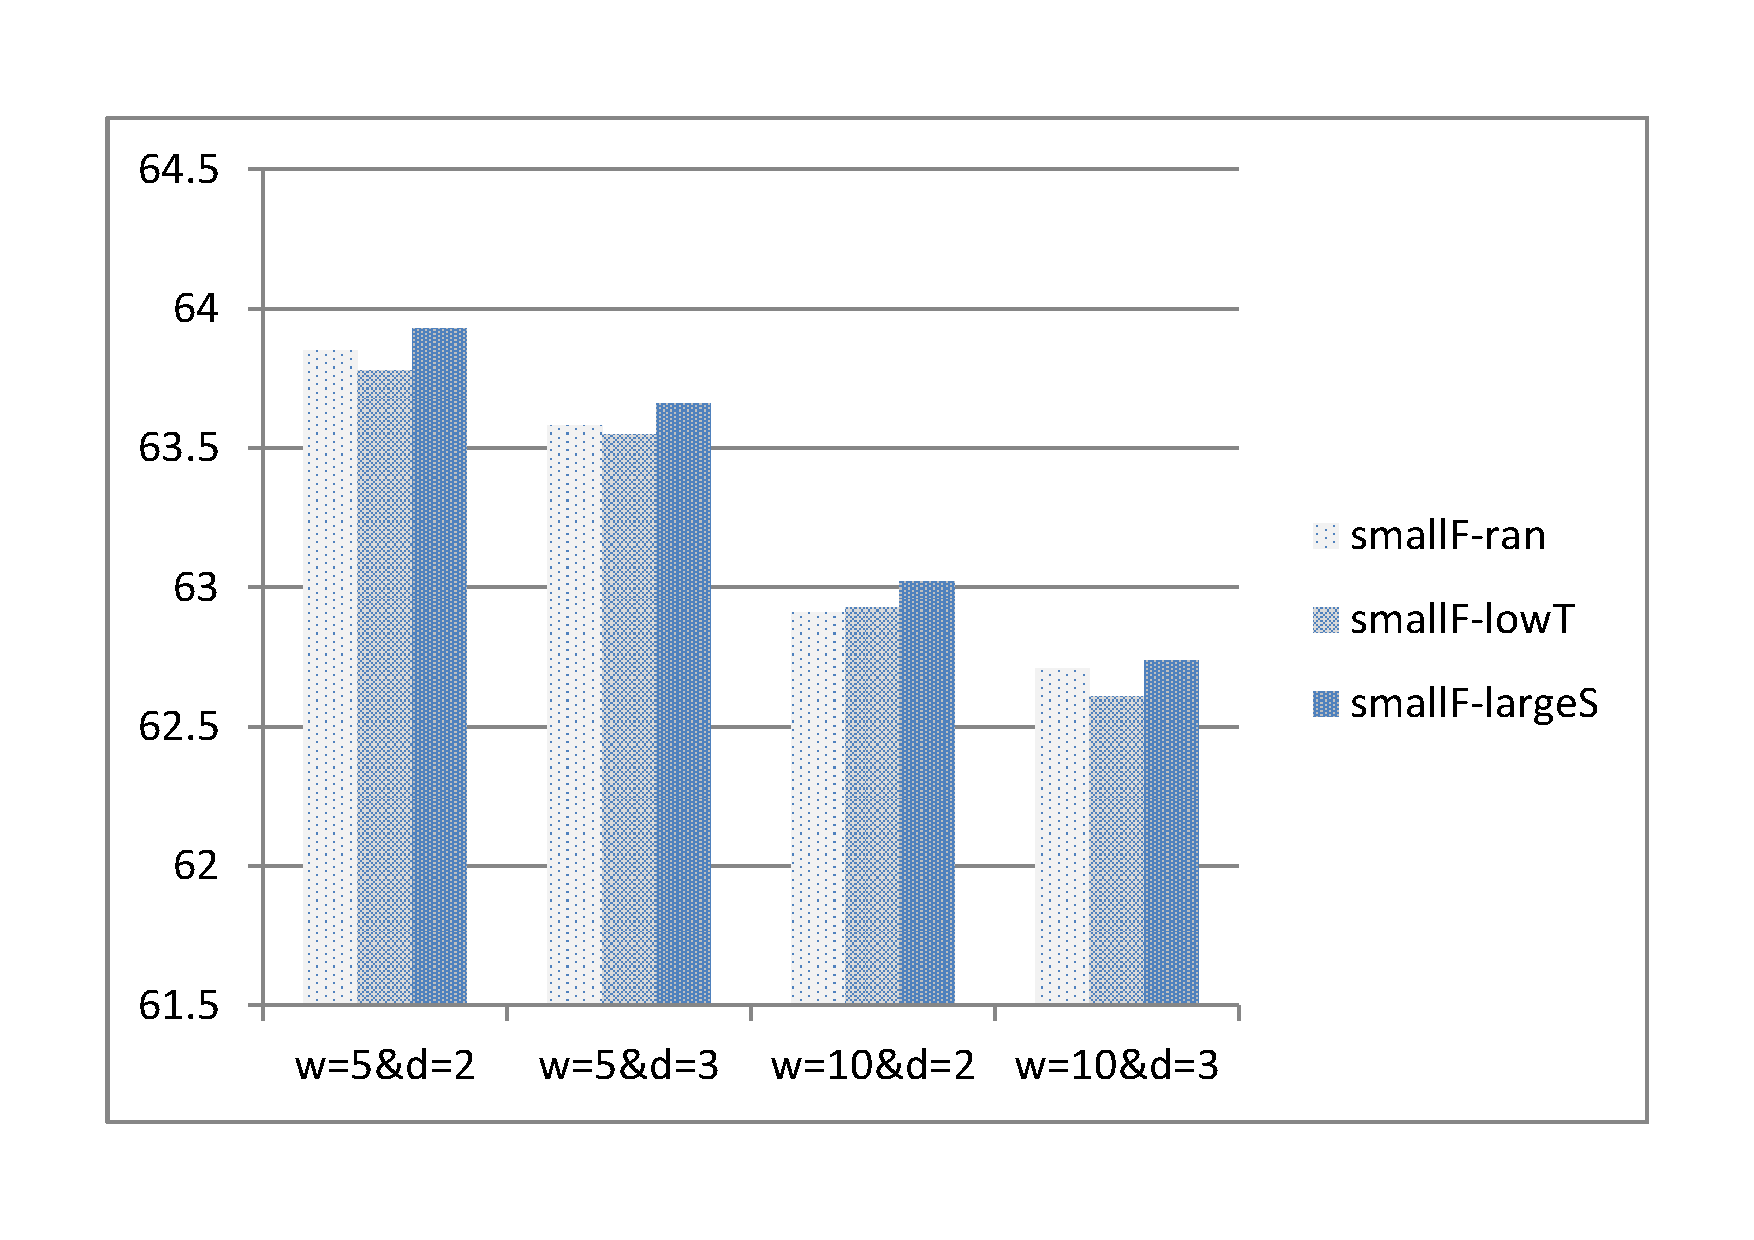
\includegraphics[width=0.4\textwidth]{fig7.pdf}
\caption{Effectiveness of evaluation schemes}
\label{fig7}
\end{figure}

\subsubsection{Probing tree size and beam width}

Next, the effect of probing tree size (width and depth) and beam width on algorithm performance is tested.
In this experiment, the evaluation scheme is set to be \texttt{smallF-lowT}.
The probing tree width is set equal to the beam width that varies from 2 to 20; $w=1$ is neglected because algorithms deteriorate to TGH when $w=1$.
The computational time increases exponentially when the probing tree depth increases, thus, the depth is only set to 1, 2, 3, or 4.
BF is classified into four categories based on the number of stacks and stack height (refer to Table \ref{tab:bf}).
The first category is the first eight data groups BF1$\sim$BF8 that have 16 stacks and 5 tiers in each instance.
The second category is BF9$\sim$BF16 with 16 stacks and 8 tiers in each instance.
The third category BF17$\sim$BF24 has 20 stacks and 5 tiers in each instance.
At last, the fourth category BF25$\sim$BF32 has 20 stacks and 8 tiers in each instance.

The performance of BS-G on the four categories is shown separately in Figures \ref{fig8:1} to \ref{fig8:4}.
Each figure shows the average number of movements of the corresponding data category obtained by BS-G for different widths and depths.
The four categories have the same trend: when search width and depth increase, performance increases, but the improvement is decreasing. Furthermore, the performance of $d=2$, $d=3$ and $d=4$ are similar, which indicates that the successor generation method is considerably precise.
Comparing Figures \ref{fig8:1} and \ref{fig8:2} with Figures \ref{fig8:3} and \ref{fig8:4}, the performance difference of different parameter combinations on BF1$\sim$BF8 and BF17$\sim$BF24 is tiny, whereas for BF9$\sim$BF16 and BF25$\sim$BF32, the performance difference is large.
BF1$\sim$BF8 and BF17$\sim$BF24 are almost solved to the optimality even with a small depth and width (see Table \ref{tab:bf}).
BF1$\sim$BF8 and BF17$\sim$BF24 are with $H=5$, whereas BF9$\sim$BF16 and BF25$\sim$BF32 are with $H=8$; all the categories have the same usage ratio.
It suggests that the height limit affects instance difficulty more than the number of stacks, because containers piled vertically are harder to retrieve than those piled horizontally.

\begin{figure*}[!htb]
\centering
\subfigure[BF1$\sim$8 average]{
    \label{fig8:1}
    \resizebox{0.4 \textwidth}{!}{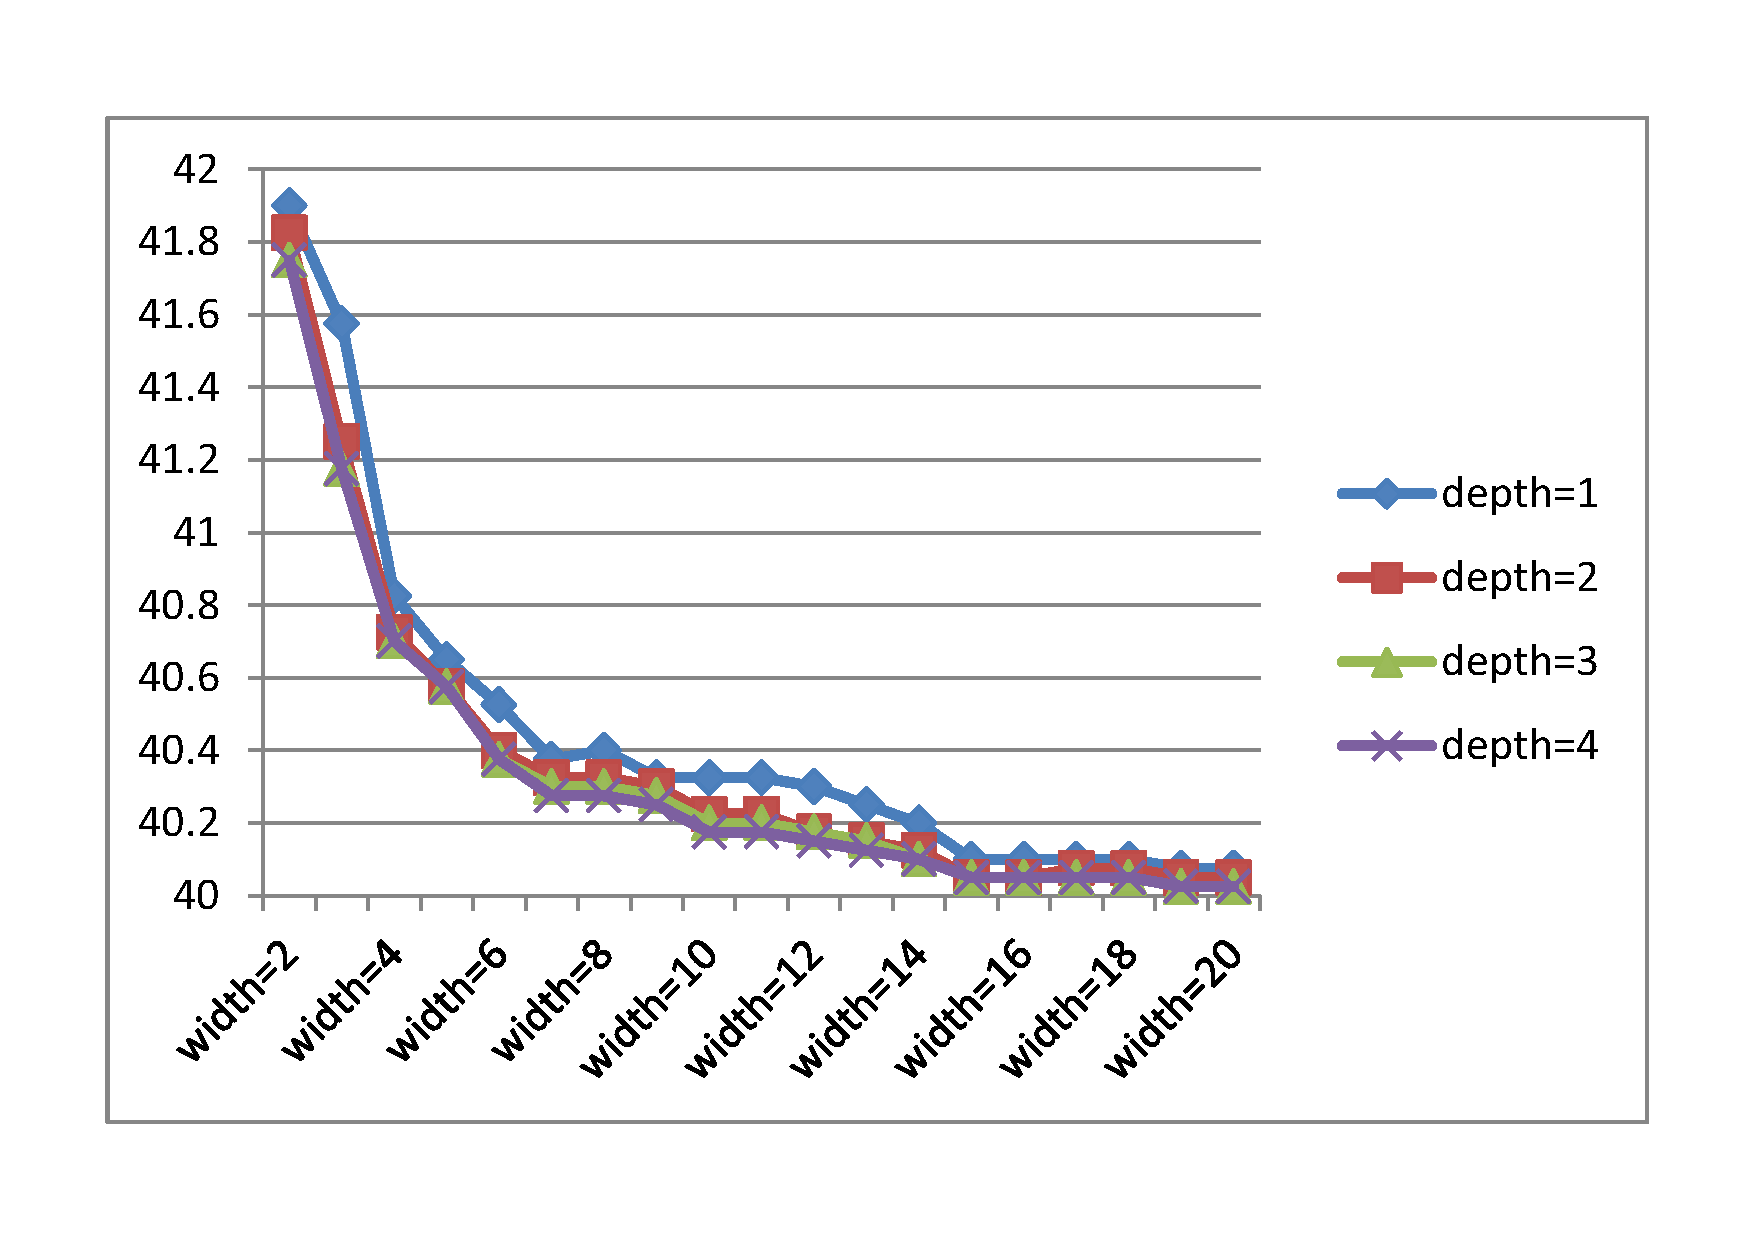
\includegraphics{fig8_1.pdf}}}
\subfigure[BF17$\sim$24 average]{
    \label{fig8:2}
    \resizebox{0.4 \textwidth}{!}{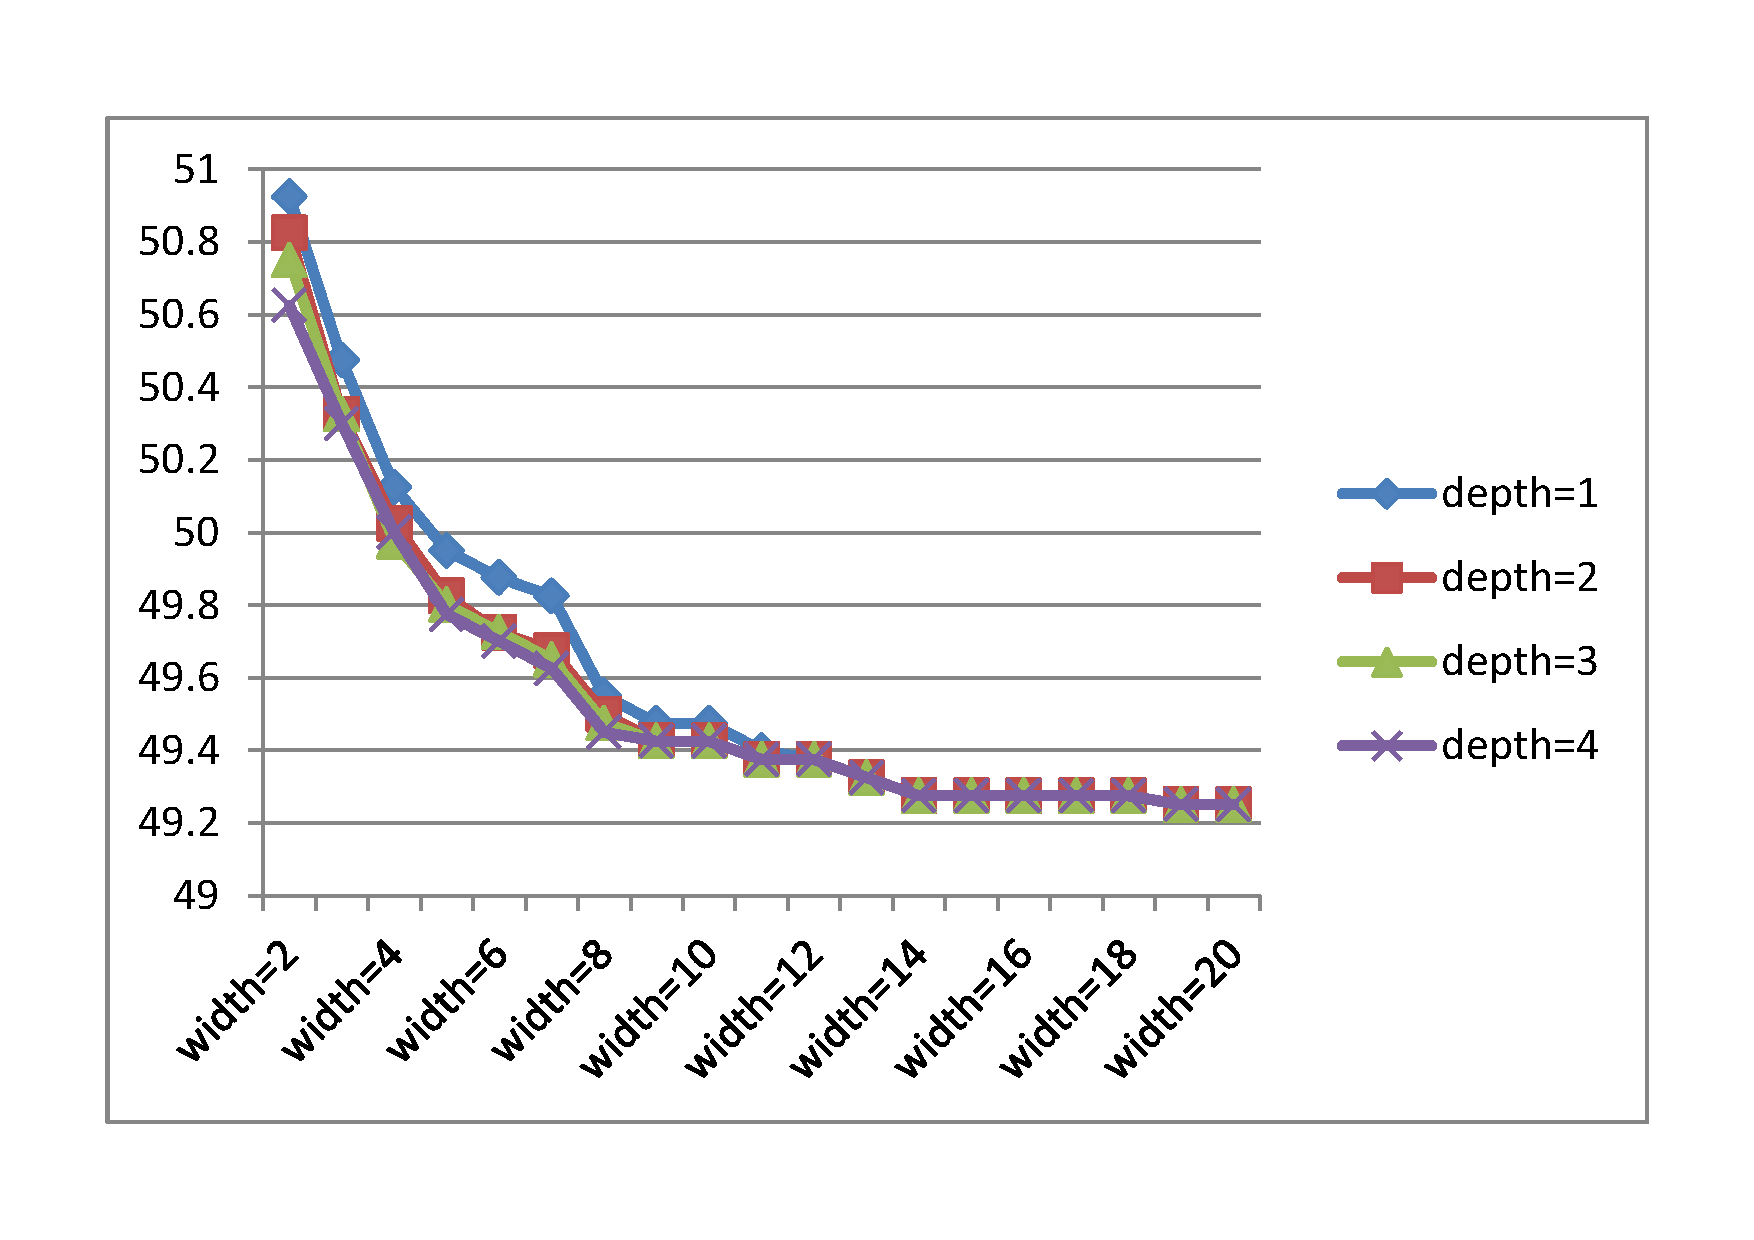
\includegraphics{fig8_2.pdf}}}
\subfigure[BF9$\sim$16 average]{
    \label{fig8:3}
    \resizebox{0.4 \textwidth}{!}{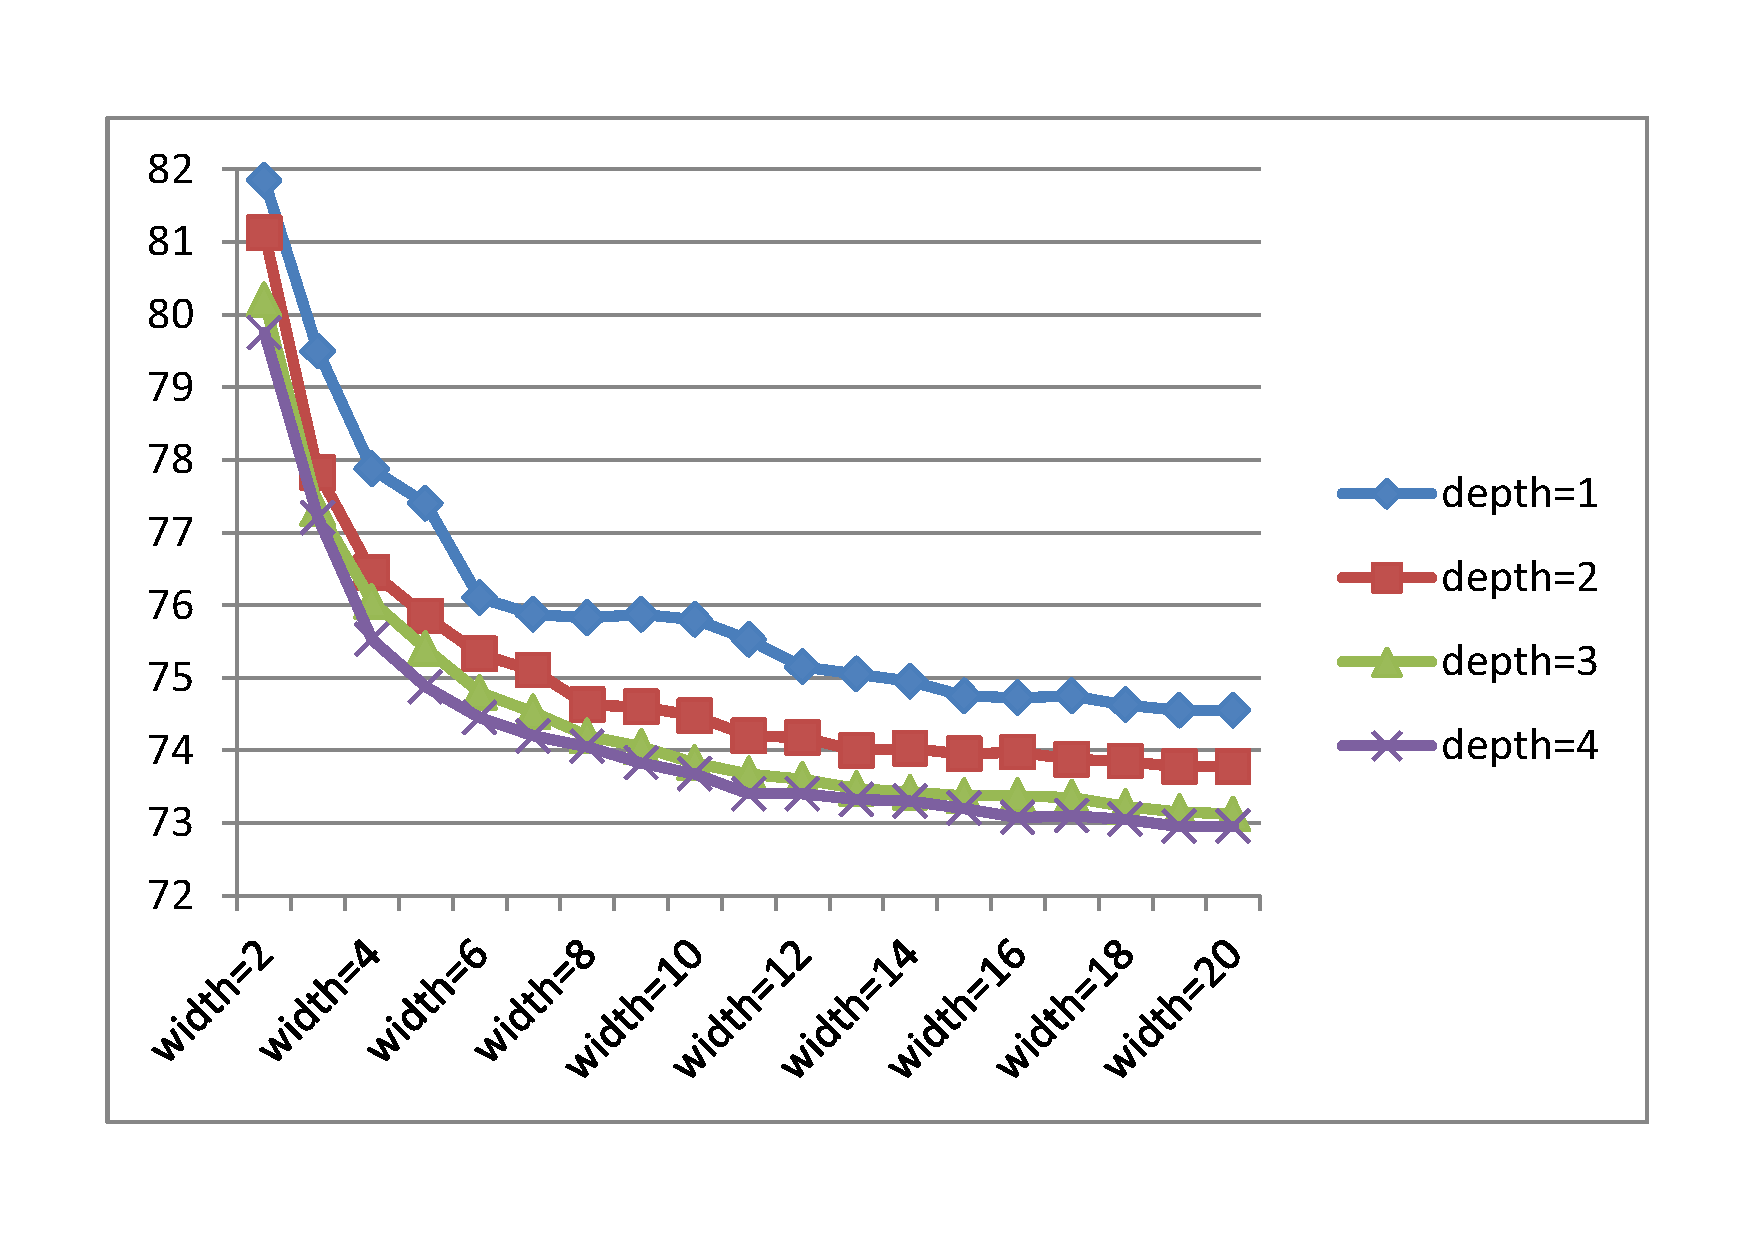
\includegraphics{fig8_3.pdf}}}
\subfigure[BF25$\sim$32 average]{
    \label{fig8:4}
    \resizebox{0.4 \textwidth}{!}{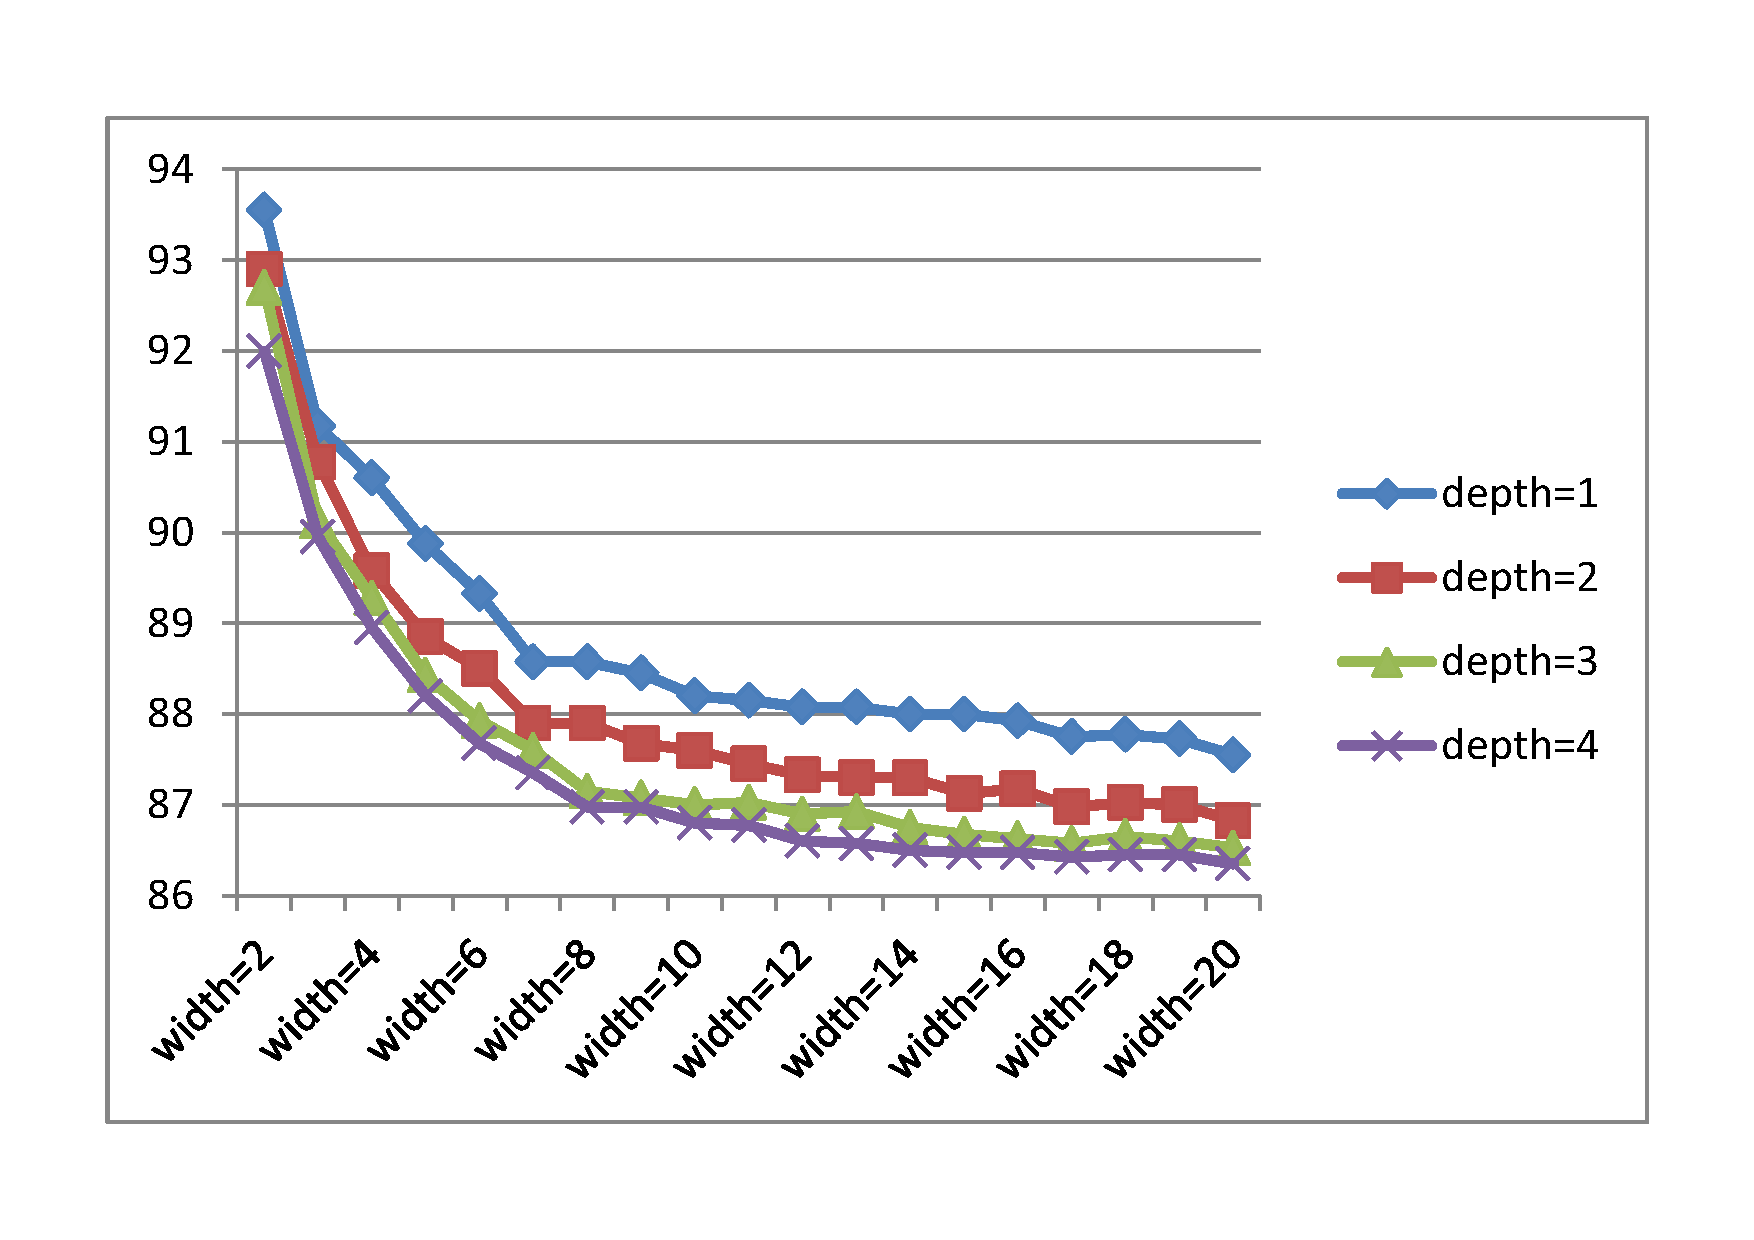
\includegraphics{fig8_4.pdf}}}
\caption{Effect of BS-G's search depth and width}
\label{fig8}
\end{figure*}

The performance of BS-B on the four categories is displayed in Figure \ref{fig9}. Its trend is similar to that of BS-G in Figure \ref{fig8}; the algorithm becomes stable and the improvement decreases as parameters increase.
However, the performance sometimes returns to a larger value as the width increases, especially when the depth is small.
For example, in Figure \ref{fig9:4}, the performance of $w=8$ \& $d=1$ is better than the performance of $w=10$ \& $d=1$.
The explanation is the algorithm degenerates to evaluate successors by TGH when $d=1$.
A smaller depth leads to a weaker ability of BS-B to evaluate successors; therefore, performance deterioration is observed.
When the search depth increases, performance deterioration disappears.
This phenomenon indicates that heuristic TGH alone is not enough to evaluate successors precisely, and incorporating probing tree search is necessary.

\begin{figure*}[!htb]
\centering
\subfigure[BF1$\sim$8 average]{
    \label{fig9:1}
    \resizebox{0.4 \textwidth}{!}{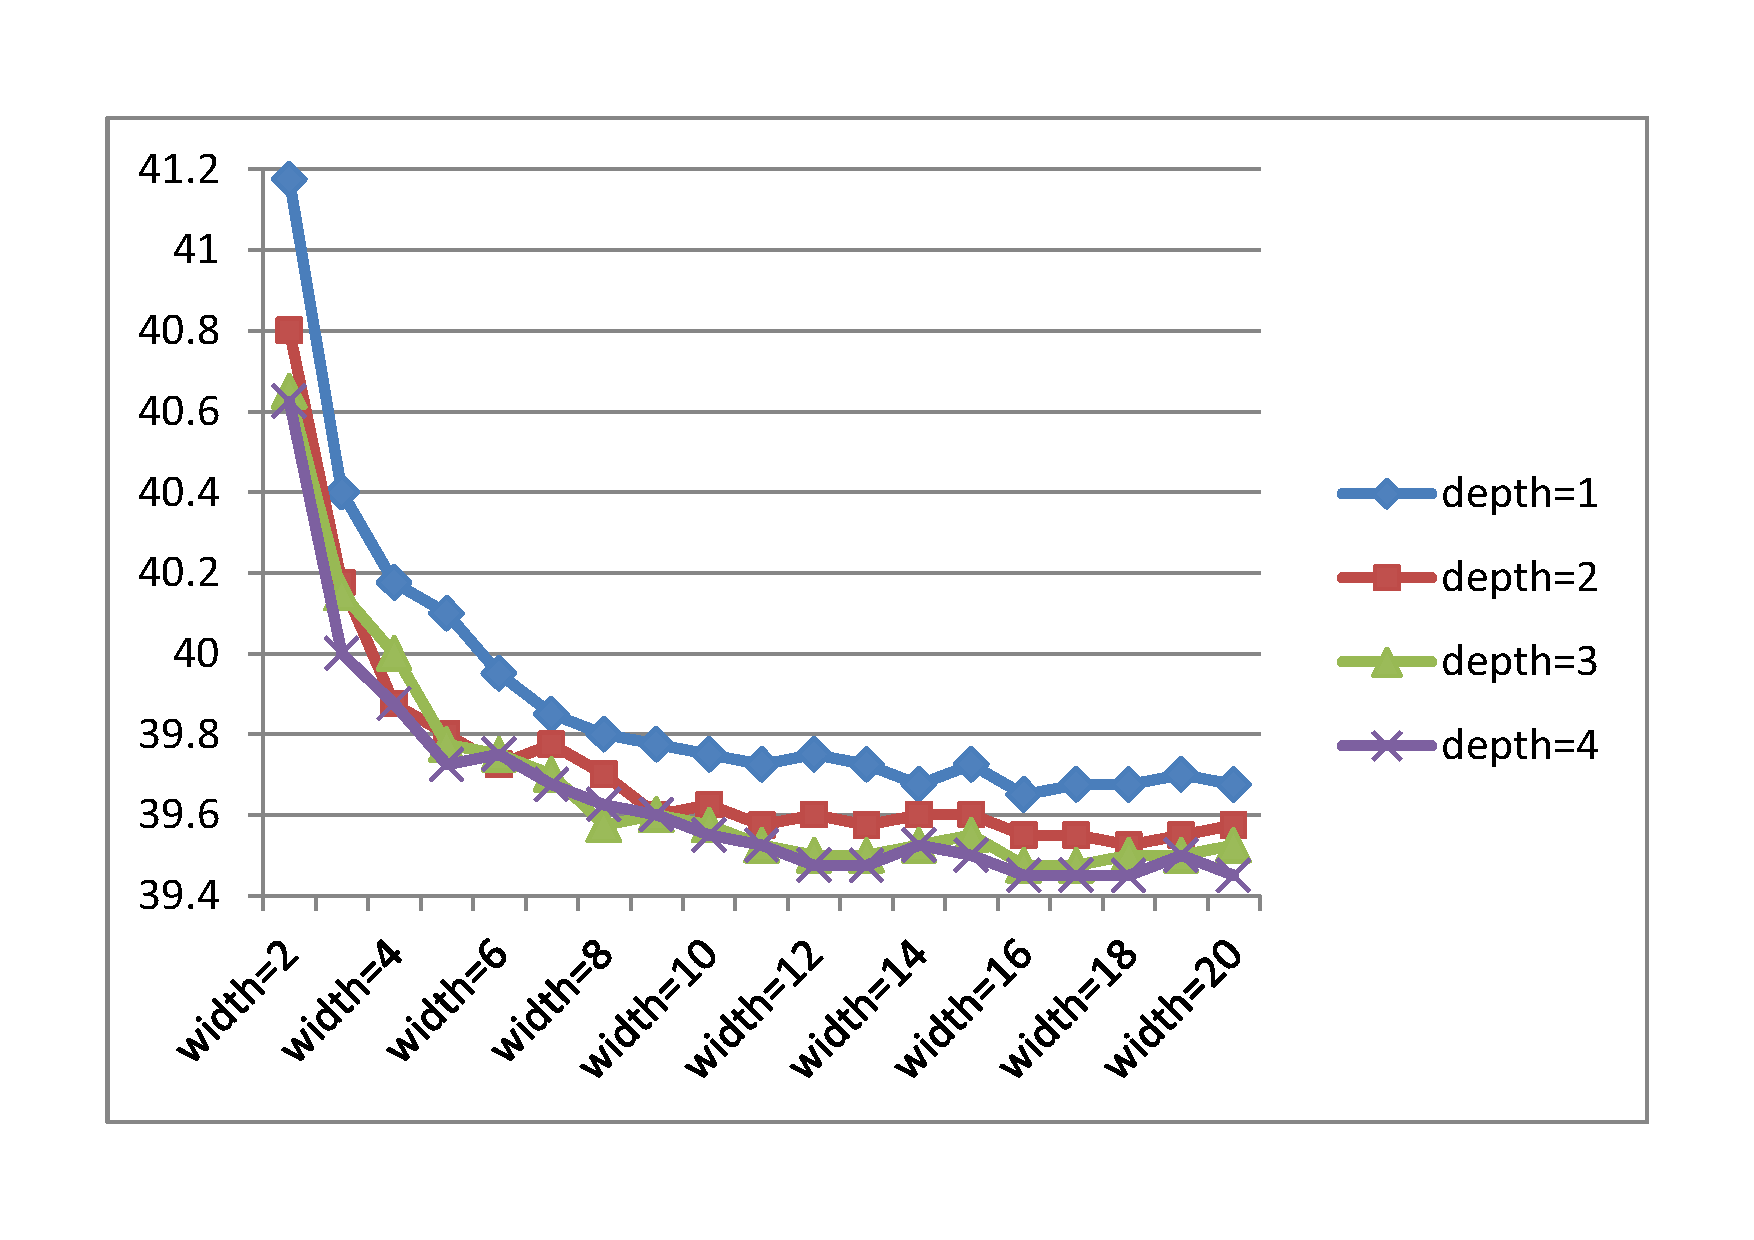
\includegraphics{fig9_1.pdf}}}
\subfigure[BF17$\sim$24 average]{
    \label{fig9:2}
    \resizebox{0.4 \textwidth}{!}{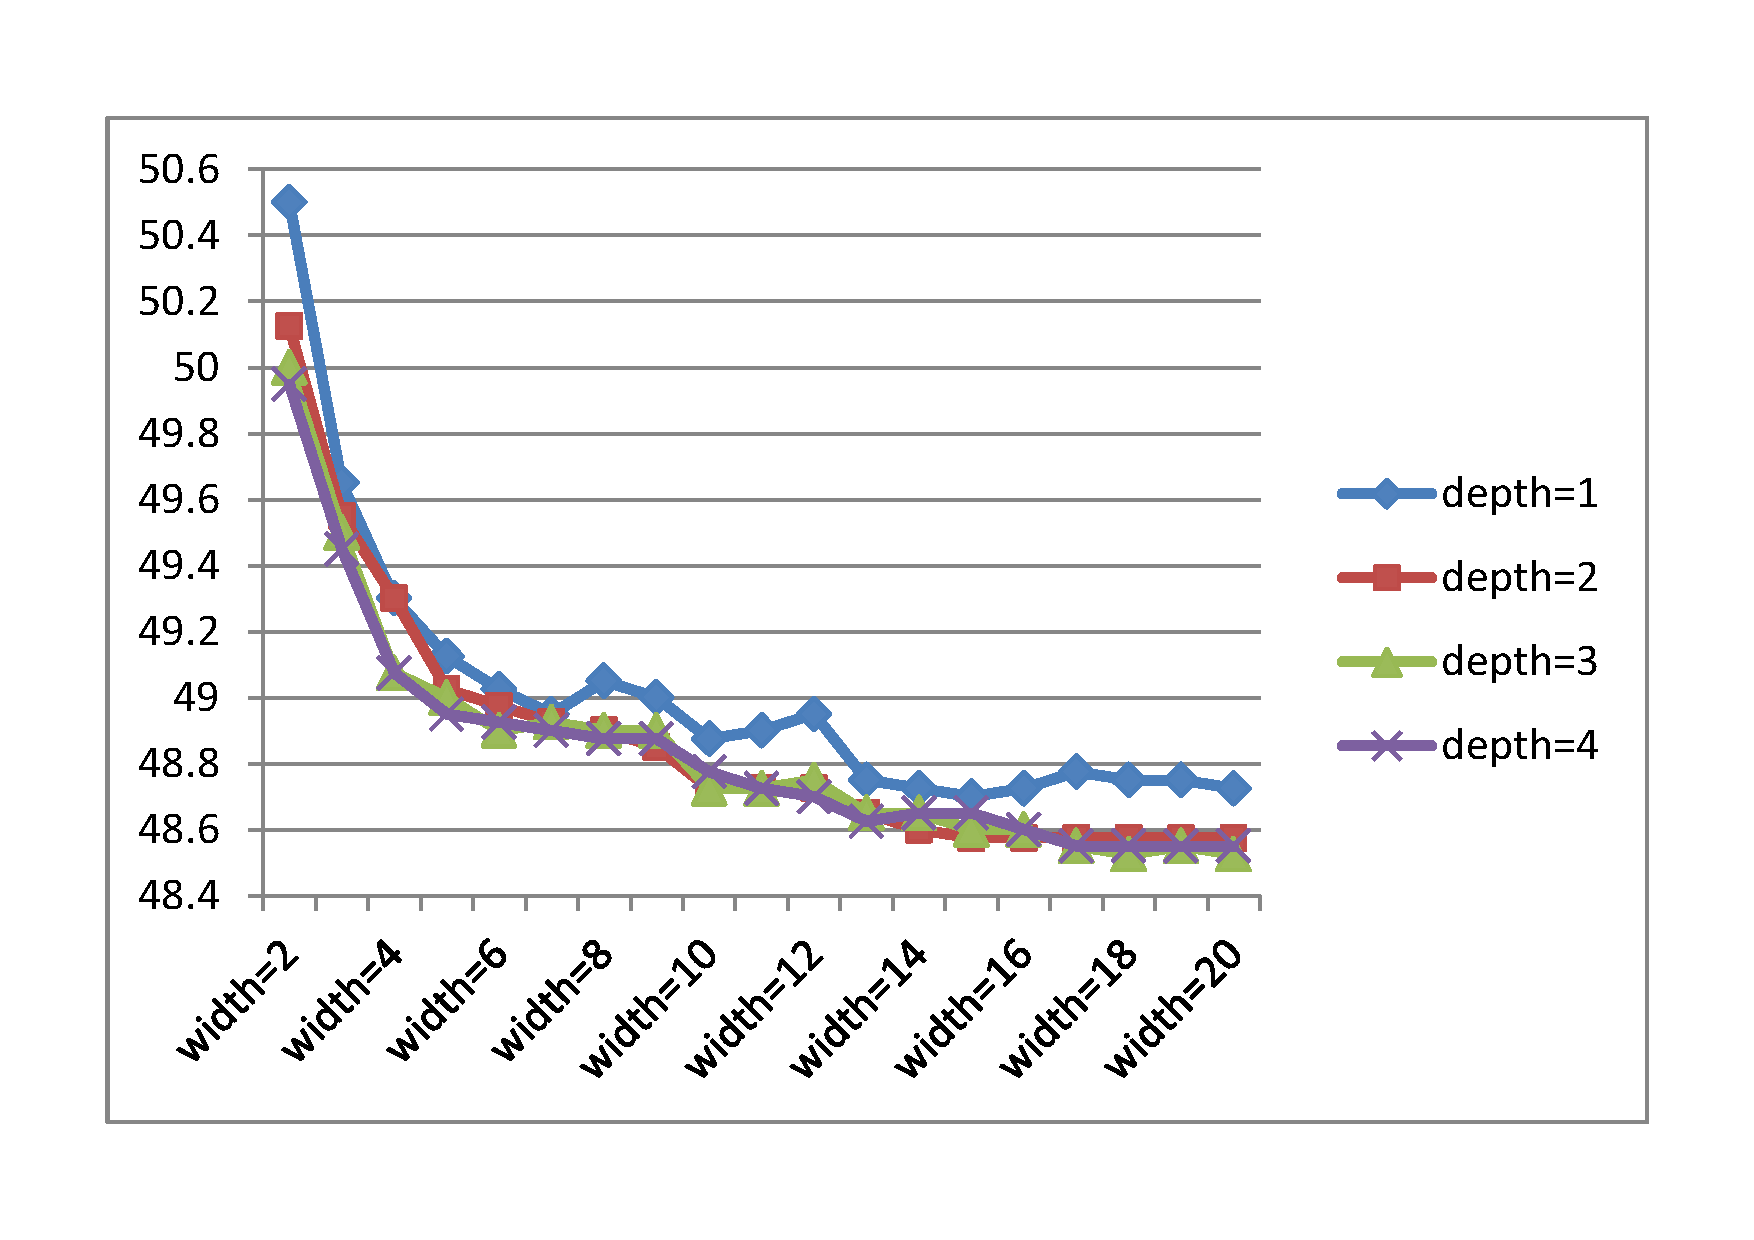
\includegraphics{fig9_2.pdf}}}
\subfigure[BF9$\sim$16 average]{
    \label{fig9:3}
    \resizebox{0.4 \textwidth}{!}{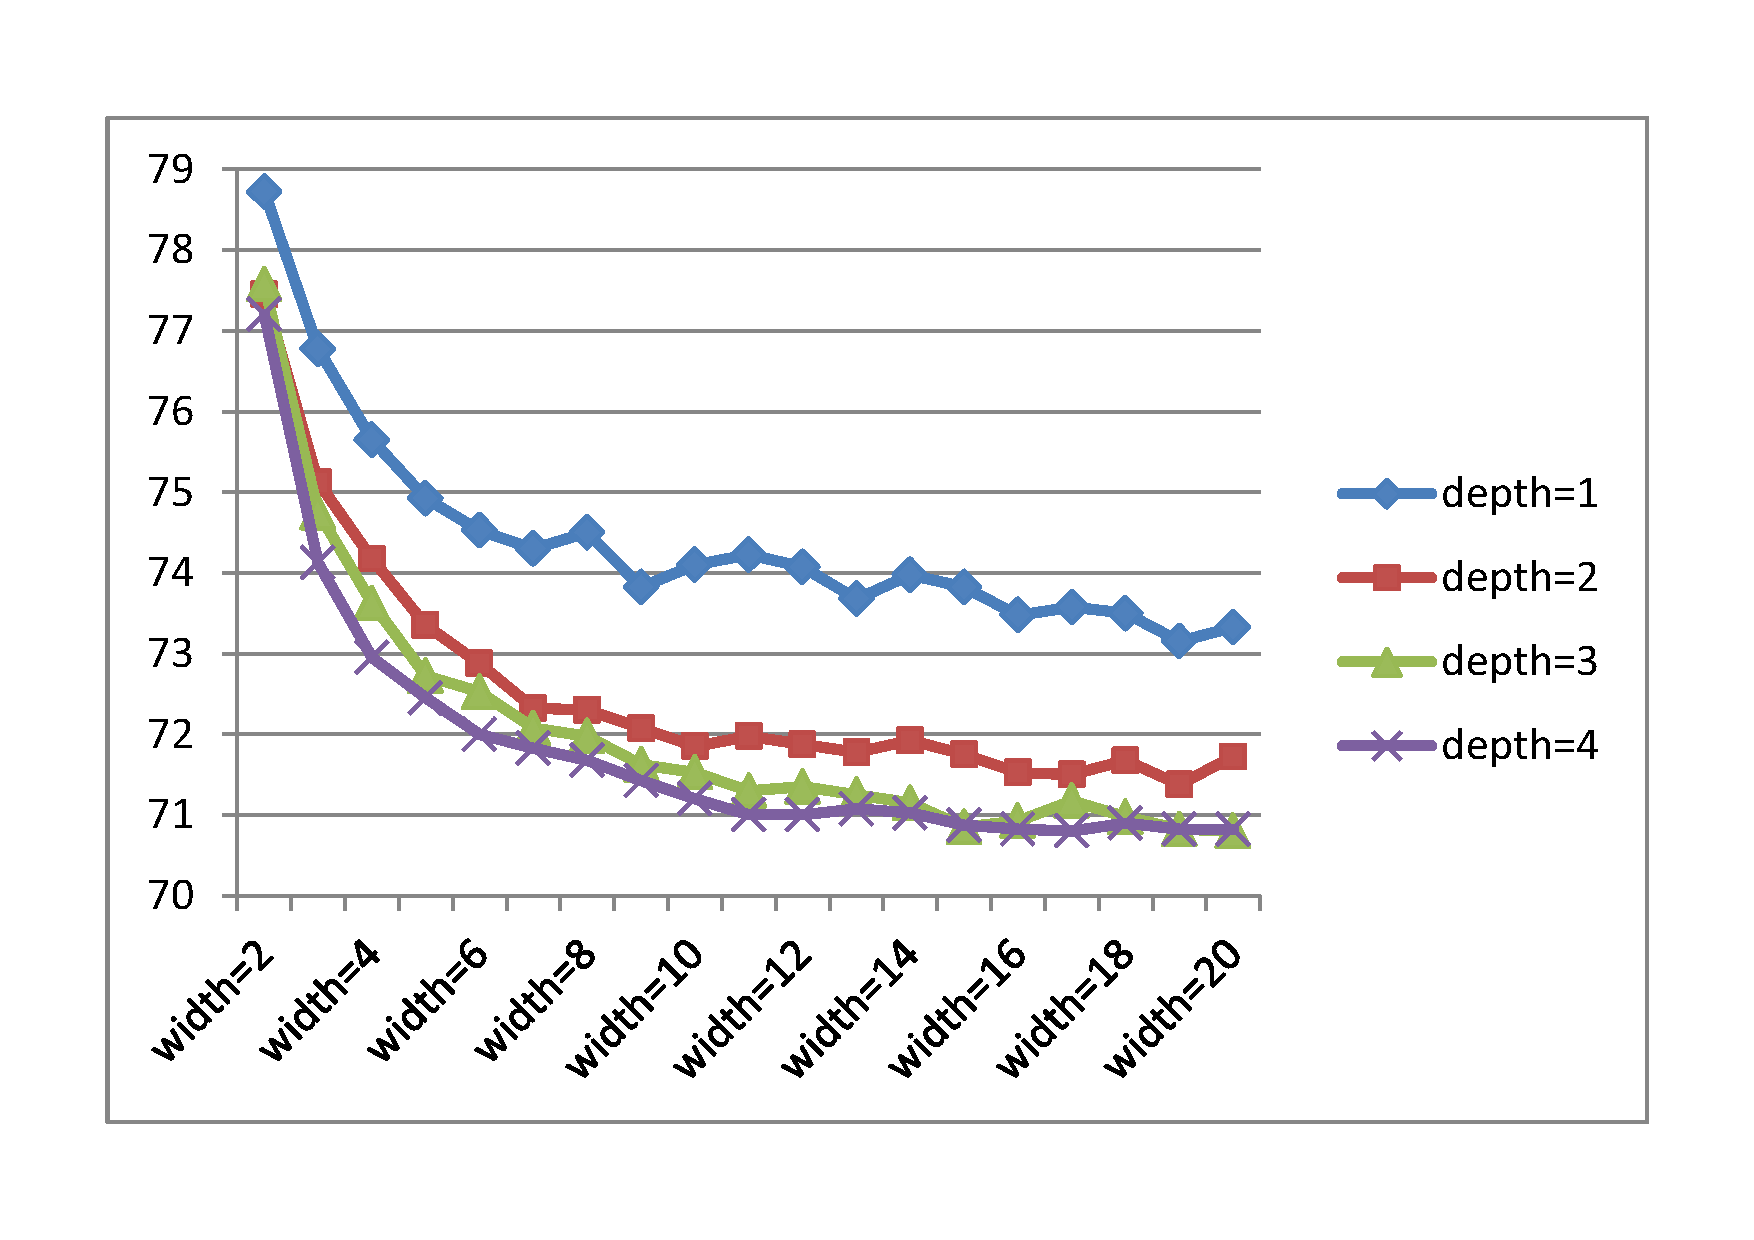
\includegraphics{fig9_3.pdf}}}
\subfigure[BF25$\sim$32 average]{
    \label{fig9:4}
    \resizebox{0.4 \textwidth}{!}{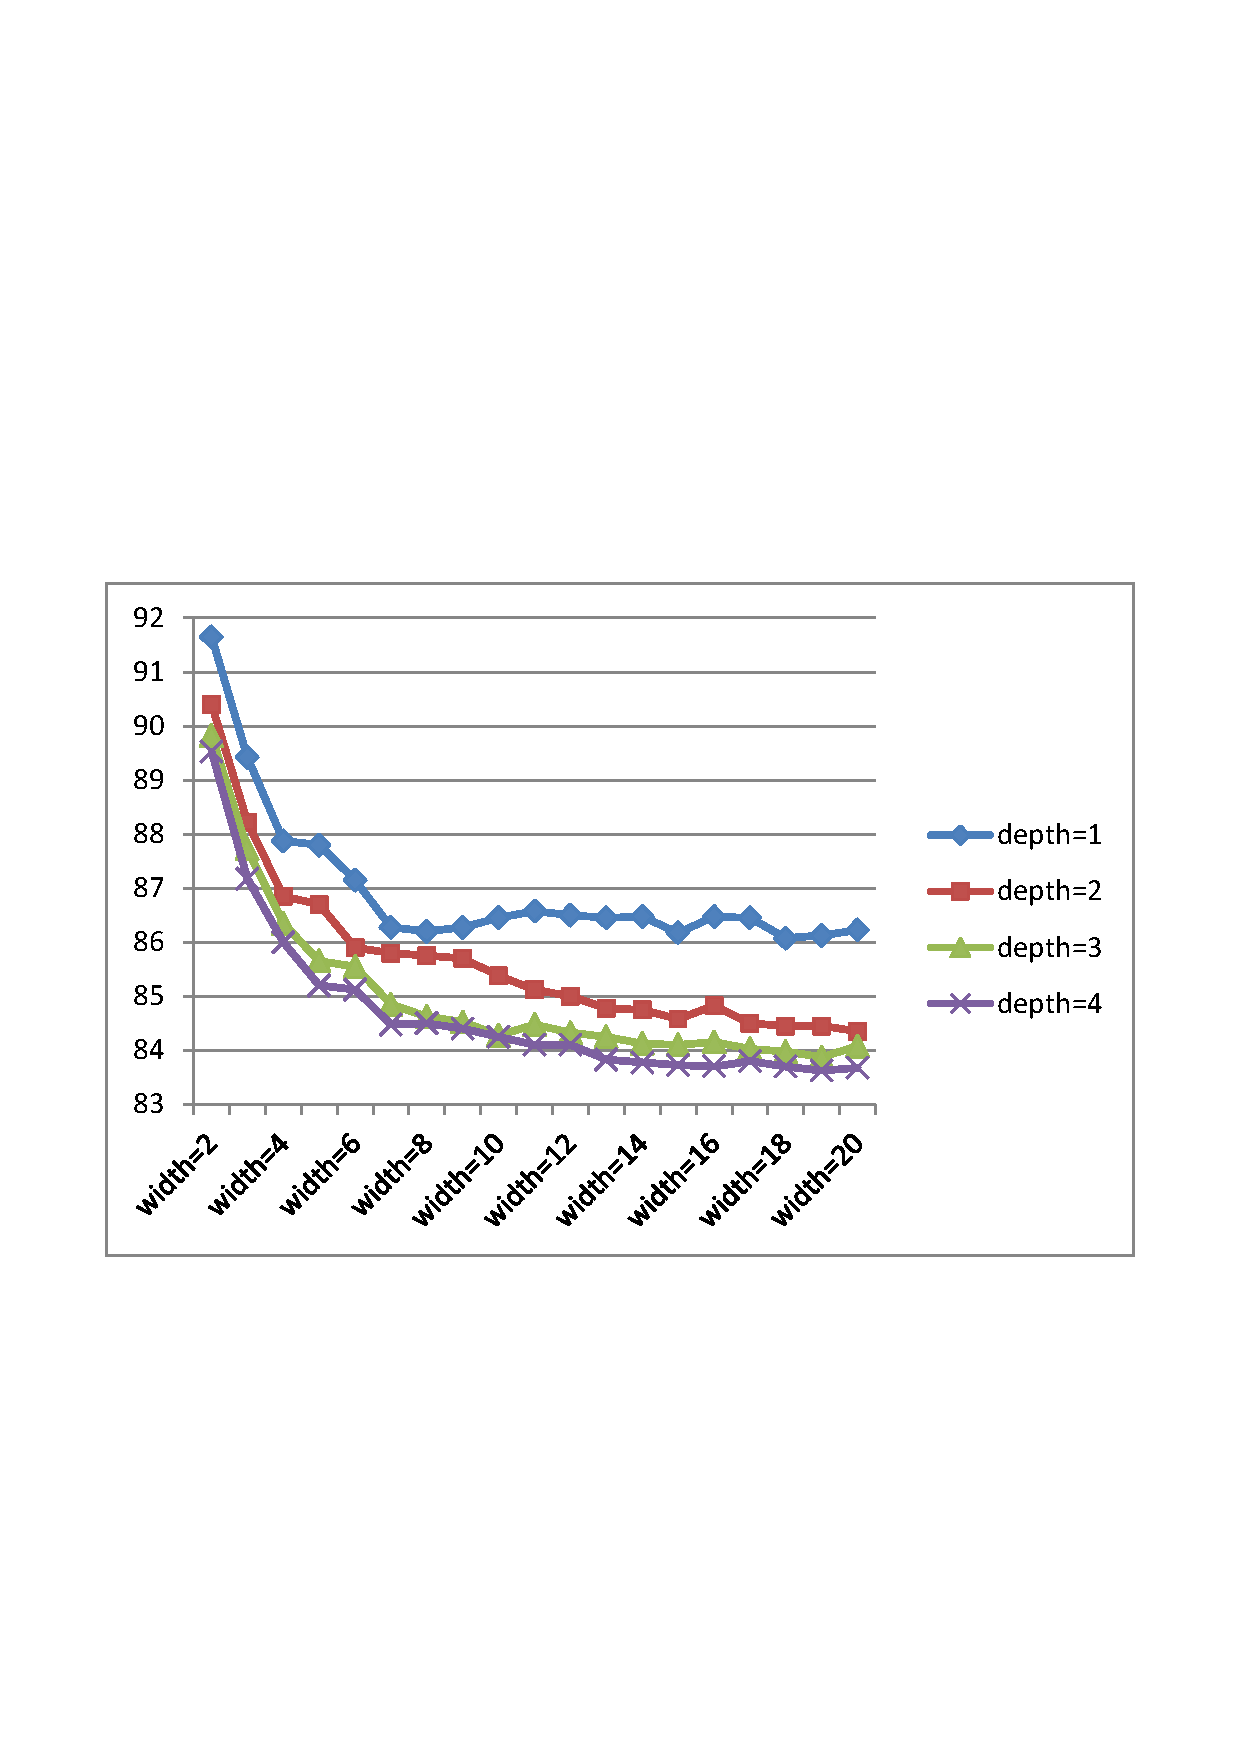
\includegraphics{fig9_4.pdf}}}
\caption{Effect of BS-B's search depth and width}
\label{fig9}
\end{figure*}

\subsection {Comparison with the existing approach}

The proposed algorithms were compared with the tree search algorithm by \cite{BF2012} (hereafter BF2012 for short) on the CPMP benchmark data.
BF2012 has the best performance on the CPMP data.
The environment of BF2012 is Intel Core 2 Duo processor (P7350, 16 GFLOPS) with 2 GHz and 2 GB RAM under Mac OS X and code was written in C and compiled with XCode under Mac OS X.
In the algorithms proposed in this paper, parameters of BS-G and BS-B are set to $\mathit{bw}=\mathit{tw}=20$ and $\mathit{td}=3$, since BS-G and BS-B become stable and the improvement is negligible if parameters increase, as shown in Figure \ref{fig8} and Figure \ref{fig9}.

To begin with, the result of data set LC mentioned in Section 7.2 of \cite{BF2012} is shown.
LC is first generated by \cite{Lee2009}, but the concrete data set is not available.
Hence, \cite{BF2012} generated a new set of instances according to the description of \cite{Lee2009}.
The result of LC is shown in Table \ref{tab:lc}, where the first five columns summarize data information copied from \cite{BF2012}.
The dirty ratio is the number of dirty containers in the initial layout divided by the number of total containers.
Columns BF2012, TGH, BS-G and BS-B are the average movements on each data group by the respective algorithms.
The average run time in seconds by BF2012, BS-G and BS-B is reported in columns tBF2012, tBS-G and tBS-B, respectively.
The run time of TGH is omitted from the table because it is less than 0.2s.
Column $\mathit{LB}_\mathit{DFS}$ indicates the average lower bounds $\mathit{LB}_\mathit{DFS}$ on each data group and column gap is the gap between BS-B and $\mathit{LB}_\mathit{DFS}$.
The last row of the table shows the mean number of movements on LC.
When calculating average time, times with ``$<1$''  and ``$<0.1$" are regarded as 1 and 0.1 s, respectively.
Those results that our algorithms outperform BF2012 are highlighted in bold.
Algorithms TGH and BS-G are worse than BF2012, whereas BS-B is better than BF2012.
However, the improvement is minimal, because the size of test instances is too small and BF2012 has almost solved the instances to the optimality, which can be inferred from the absolute spread between lower bounds and solutions.

\begin{table*}[!htb]
\scriptsize
\centering
  \caption{\label{tab:lc} Comparison on data set LC}
    \begin{tabular}{c|c|c|c|c|c|c|c|c|c|c|c|c|c}

    \hline
    group & stack & height & usage rate & dirty ratio & BF2012 & tBF2012 & TGH   & BS-G  & tBS-G & BS-B  & tBS-B & $\mathit{LB}_\mathit{DFS}$ & gap\\
    \hline
    LC1   & 10   & 5  & 0.7  & 0.37 & 17   & $<1$ & 22   & 17         & $<0.1$ & 17             & $<1$  & 15 & 13.33\%\\
    LC2a  & 12   & 6  & 0.69 & 0.38 & 22.6 & 1    & 26.9 & 23.2       & $<0.1$ & \textbf{22.3}  & $<1$  & 21.1 & 5.69\%\\
    LC2b  & 12   & 6  & 0.69 & 0.7  & 38.4 & 2.1  & 46.7 & \textbf{38}& $<0.1$ & \textbf{37.9}  & 1.37  & 37.3 & 1.61\%\\
    LC3a  & 12   & 6  & 0.75 & 0.39 & 23.7 & 1.4  & 29.1 & 23.9       & $<0.1$ & 23.7           & $<1$  & 22.3 & 6.28\%\\
    LC3b  & 12   & 6  & 0.75 & 0.67 & 42.7 & 4.2  & 54.8 & 43.6       & $<1$   & \textbf{42.3}  & 10.33 & 39.9 & 6.02\%\\
    \hline
    Ave   & 11.6 & 5.8& 0.72 & 0.5  & 28.88& 1.94 & 35.9 & 29.14      & $<1$   & \textbf{28.64} & 2.69  & 27.12&
    5.6\% \\
    \hline
    \end{tabular}%
\end{table*}%

Then the proposed algorithms were compared with BF2012 on data set CV.
CV is provided by \cite{Caserta2009} and \cite{BF2012} has the best performance on it.
Table \ref{tab:cv} illustrates the comparative result that both BS-G and BS-B surpass BF2012.

\begin{table*}[!htb]
\scriptsize
  \centering
  \caption{\label{tab:cv} Comparison on data set CV}
    \begin{tabular}{c|c|c|c|c|c|c|c|c|c|c|c|c|c}
    \hline
    group & stack & height & usage rate & dirty ratio & BF2012 & tBF2012 & TGH   & BS-G  & tBS-G & BS-B  & tBS-B & $\mathit{LB}_\mathit{DFS}$ & gap\\
    \hline
    CV1  & 3  & 9   & 0.33 & 0.6  & 10.5 & $<1$ & 12.1 & 10.6          & $<0.01$ & \textbf{10}   & $<0.01$ &7.9 & 26.58\%\\
    CV2  & 4  & 16  & 0.25 & 0.66 & 19.1 & $<1$ & 20.3 & \textbf{17.8} & $<0.01$ & \textbf{17.2} & $<0.1$ &13.6 & 26.47\%\\
    CV3  & 5  & 25  & 0.2  & 0.7  & 30.4 & 9.1  & 34   & \textbf{27.3} & $<0.1$  & \textbf{26.4} & $<1$   &21.3 & 23.94\%\\
    CV4  & 6  & 36  & 0.17 & 0.74 & 44.4 & 20   & 50   & \textbf{37.1} & $<0.1$  & \textbf{35.9} & $<1$   &28.1 & 27.76\%\\
    \hline
    Ave  & 4.5& 21.5& 0.24 & 0.67 & 26.1 & 7.78 & 29.1 & \textbf{23.2} & $<0.1$  & \textbf{22.38}& $<1$   & 17.73 & 26.23\%\\
    \hline
    \end{tabular}%
\end{table*}%

Finally, the result of data set BF is shown in Table \ref{tab:bf}. BF is generated by \cite{BF2012}; the produced instances are supposedly difficult enough to justify the performance of algorithms. The performance of TGH is worse than that of BF2012 because BF2012 deploys a tree search algorithm, whereas TGH is only a greedy heuristic. BS-G and BS-B outperform BF2012 by almost 5\% and 7\%, respectively.


\begin{table*}[!htb]
\caption{\label{tab:bf} Comparison on data set BF}
\scriptsize
\centering
\begin{tabular}{c|c|c|c|c|c|c|c|c|c|c|c|c|c}
  \hline
  group & stack & height & usage rate & dirty ratio & BF2012 & tBF2012 & TGH   & BS-G  & tBS-G & BS-B  & tBS-B & $\mathit{LB}_\mathit{DFS}$ & gap\\
    \hline
    BF1   & 16 & 5  & 0.6 & 0.6  & 29.1  & $<1$  & 29.1   & 29.1          & $<0.01$ & 29.1           & $<0.01$ & 29.1  & 0\\
    BF2   & 16 & 5  & 0.6 & 0.75 & 36    & $<1$  & 36     & 36            & $<0.01$ & 36             & $<0.01$ & 36    & 0\\
    BF3   & 16 & 5  & 0.6 & 0.6  & 29.1  & $<1$  & 29.45  & 29.15         & $<0.01$ & 29.1           & $<0.1$  & 29.1  & 0\\
    BF4   & 16 & 5  & 0.6 & 0.75 & 36    & $<1$  & 36     & 36            & $<0.01$ & 36             & $<0.01$ & 36    & 0\\
    BF5   & 16 & 5  & 0.8 & 0.61 & 41.6  & 8     & 48.25  & 42.05         & $<0.1$  & \textbf{41.35} & 3.73    & 40.75 & 1.47\%\\
    BF6   & 16 & 5  & 0.8 & 0.75 & 49.4  & 4.9   & 57.65  & 51.1          & $<0.1$  & 50.15          & 10.87   & 48.6  & 3.19\%\\
    BF7   & 16 & 5  & 0.8 & 0.61 & 42.9  & 26.3  & 53.5   & 44.75         & $<0.1$  & 43.05          & 8.95    & 41.3  & 4.24\%\\
    BF8   & 16 & 5  & 0.8 & 0.75 & 50.6  & 24.7  & 60.05  & 51.95         & $<0.1$  & 51.15          & 15.75   & 49.05 & 4.28\%\\
    BF9   & 16 & 8  & 0.6 & 0.61 & 51.8  & 30.8  & 60.35  & \textbf{51.5} & $<0.1$  & \textbf{50.4}  & 6.87    & 49.35 & 2.13\%\\
    BF10  & 16 & 8  & 0.6 & 0.75 & 59.8  & 21.9  & 62.05  & \textbf{58.9} & $<0.01$ & \textbf{58.75} & 2.99    & 58.4  & 0.6\%\\
    BF11  & 16 & 8  & 0.6 & 0.61 & 52.2  & 44.6  & 61.15  & 52.3          & $<0.1$  & \textbf{51.15} & 7.75    & 49.25 & 3.86\%\\
    BF12  & 16 & 8  & 0.6 & 0.75 & 60.2  & 28.2  & 63.45  & \textbf{59.2} & $<0.1$  & \textbf{58.65} & 3.47    & 58.2  & 0.77\%\\
    BF13  & 16 & 8  & 0.8 & 0.6  & 84.6  & 60    & 107.45 & \textbf{79.75}& 2.67    & \textbf{75.4}  & 167.50  & 65.95 & 14.33\%\\
    BF14  & 16 & 8  & 0.8 & 0.76 & 105.6 & 60    & 125.25 & \textbf{96.3} & 4.62    & \textbf{93.1}  & 293.56  & 81.25 & 14.58\%\\
    BF15  & 16 & 8  & 0.8 & 0.6  & 95.5  & 60    & 110.9  & \textbf{82.8} & 2.66    & \textbf{78.7}  & 176.51  & 65.85 & 19.51\%\\
    BF16  & 16 & 8  & 0.8 & 0.76 & 109.8 & 60    & 133.3  & \textbf{98}   & 4.28    & \textbf{93.55} & 275.25  & 81.75 & 14.43\%\\
    BF17  & 20 & 5  & 0.6 & 0.6  & 36.3  & 3.5   & 36.45  & \textbf{36.25}& $<0.01$ & \textbf{36.25} & $<0.01$ & 36.25 & 0\\
    BF18  & 20 & 5  & 0.6 & 0.75 & 45    & $<1$  & 45     & 45            & $<0.01$ & 45             & $<0.01$ & 45    & 0\\
    BF19  & 20 & 5  & 0.6 & 0.6  & 36.5  & $<1$  & 36.8   & 36.5          & $<0.01$ & \textbf{36.45} & $<0.01$ & 36.45 & 0\\
    BF20  & 20 & 5  & 0.6 & 0.75 & 45    & $<1$  & 45     & 45            & $<0.01$ & 45             & $<0.01$ & 45    & 0\\
    BF21  & 20 & 5  & 0.8 & 0.6  & 51.7  & 31.5  & 60.8   & 52.45         & $<0.1$  & \textbf{51.55} & 20.31   & 50.65 & 1.78\%\\
    BF22  & 20 & 5  & 0.8 & 0.75 & 60.9  & 7.6   & 68.9   & 62.85         & $<0.1$  & 61.8           & 14.47   & 60.65 & 1.9\%\\
    BF23  & 20 & 5  & 0.8 & 0.6  & 51.5  & 25.5  & 60.85  & 52.4          & $<0.1$  & \textbf{50.95} & 13.90   & 50.35 & 1.19\%\\
    BF24  & 20 & 5  & 0.8 & 0.75 & 61.3  & 18.2  & 70.95  & 63.25         & $<0.1$  & 62.05          & 24.45   & 60.65 & 2.31\%\\
    BF25  & 20 & 8  & 0.6 & 0.6  & 62.8  & 45    & 69.95  & \textbf{62.1} & $<0.1$  & \textbf{61.5}  & 12.79   & 60.35 & 1.91\%\\
    BF26  & 20 & 8  & 0.6 & 0.75 & 74    & 30.8  & 74.35  & \textbf{72.6} & $<0.1$  & \textbf{72.35} & 2.53    & 72.1  & 0.35\%\\
    BF27  & 20 & 8  & 0.6 & 0.6  & 64    & 55.9  & 71.8   & \textbf{62.75}& $<0.1$  & \textbf{61.85} & 16.12   & 60.35 & 2.49\%\\
    BF28& 20 & 8  & 0.6 & 0.75 & 74.9  & 44.7  & 76.1   & \textbf{73}   & $<0.1$  & \textbf{72.65} & 5.82    & 72.35 & 0.41\%\\
    BF29  & 20 & 8  & 0.8 & 0.6  & 106.6 & 60    & 120.55 & \textbf{96.05}& 8.5     & \textbf{92.05} & 396.10  & 81.6  & 12.81\%\\
    BF30  & 20 & 8  & 0.8 & 0.75 & 128.5 & 60    & 143.05 &\textbf{ 114.3}& 11.4    & \textbf{110.25}& 581.61  & 99.65 & 10.64\%\\
    BF31  & 20 & 8  & 0.8 & 0.6  & 115.2 & 60    & 128.15 & \textbf{98.9} & 9.17    & \textbf{93.95} & 429.09  & 81.15 & 15.77\%\\
    BF32  & 20 & 8  & 0.8 & 0.75 & 132.3 & 60    & 147.3  & \textbf{115.55}& 8.32   & \textbf{111.8} & 612.55  & 99.2  & 12.7\%\\
    \hline
    Ave   & 18 & 6.5& 0.7 & 0.68 & 65.02 & 29.35 & 72.81  & \textbf{62.12}& 1.64    & \textbf{60.66} & 96.97   & 57.24 & 5.97\%\\
   \hline
\end{tabular}
\end{table*}

\subsection {Result on new data set}

A new data set for CPMPDS is generated. All the data are available upon request. %online\footnote{\url{http://www.computational-logistics.org/orlib/topic/CPMPDS/index.html}}.
The new data set is composed of 36 groups of instances with 30 instances in each group.
The number of stacks (dummy stack included) is 6, 8, or 10, which is close to the number of stacks in a bay in reality.
The maximum height limit is 5 or 8 and is restricted by material handling equipment.
Two alternatives are available with respect to the usage rate. One alternative is 60\%$\sim$80\%, and another alternative is 80\% above.
Based on \cite{BF2012}, the number of different group labels in an instance is determined by the group ratio (equal to the number of different groups divided by the number of containers).
In the new data set, the group ratio has three ranges: 100\%, 60\%$\sim$80\%, 30\%$\sim$50\%.
Particularly, a group ratio of 100\% means that the group labels of containers are unique.
The results by TGH, BS-G and BS-B are shown in Table \ref{tab:cpmpds}.

\begin{table*}[!htb]

\caption{\label{tab:cpmpds} Result on new data for the CPMPDS}
\footnotesize
\centering
\begin{tabular}{c|c|c|c|c|c|c|c|c|c}

    \hline
    group & stack & tier  & usage rate & dirty ratio & TGH   & BS-G  & tBS-G & BS-B  & tBS-B \\
    \hline
    CPMPDS1 & 6      & 5     & 0.70  & 0.57  & 29.33   & 21.13  & $<0.1$  & 19.97  & $<1$ \\
    CPMPDS2 & 6      & 5     & 0.72  & 0.62  & 33.10   & 23.30  & $<0.1$  & 21.97  & $<1$ \\
    CPMPDS3 & 6      & 5     & 0.69  & 0.53  & 23.87   & 17.83  & $<0.1$  & 17.37  & $<1$\\
    CPMPDS4 & 6      & 5     & 0.82  & 0.68  & 62.13   & 37.37  & $<0.1$  & 34.33  & $<1$ \\
    CPMPDS5 & 6      & 5     & 0.82  & 0.63  & 55.03   & 33.23  & $<1$    & 30.43  & 1.16  \\
    CPMPDS6 & 6      & 5     & 0.82  & 0.61  & 53.57   & 30.70  & $<1$    & 28.90  & 1.98  \\
    CPMPDS7 & 6      & 8     & 0.68  & 0.73  & 72.97   & 43.73  & $<1$    & 41.00  & 1.23  \\
    CPMPDS8 & 6      & 8     & 0.69  & 0.74  & 74.47   & 45.40  & $<1$    & 42.27  & 2.28  \\
    CPMPDS9 & 6      & 8     & 0.69  & 0.73  & 60.80   & 41.37  & $<1$    & 39.63  & 2.28  \\
    CPMPDS10 & 6     & 8     & 0.80  & 0.78  & 142.73  & 72.00  & $<1$    & 66.93  & 4.05  \\
    CPMPDS11 & 6     & 8     & 0.81  & 0.78  & 157.57  & 72.83  & $<1$    & 68.63  & 6.09  \\
    CPMPDS12 & 6     & 8     & 0.81  & 0.75  & 138.43  & 66.43  & $<1$    & 62.60  & 11.27  \\
    CPMPDS13 & 8     & 5     & 0.71  & 0.60  & 32.47   & 25.30  & $<0.1$  & 24.33  & $<1$ \\
    CPMPDS14 & 8     & 5     & 0.72  & 0.59  & 33.67   & 25.93  & $<1$    & 25.03  & 1.17  \\
    CPMPDS15 & 8     & 5     & 0.68  & 0.55  & 25.40   & 21.17  & $<0.1$  & 20.43  & $<1$ \\
    CPMPDS16 & 8     & 5     & 0.84  & 0.69  & 73.50   & 44.30  & $<1$    & 41.50  & 3.86  \\
    CPMPDS17 & 8     & 5     & 0.83  & 0.64  & 64.67   & 39.00  & $<1$    & 37.47  & 4.85  \\
    CPMPDS18 & 8     & 5     & 0.83  & 0.61  & 53.83   & 35.30  & $<1$    & 33.77  & 5.23  \\
    CPMPDS19 & 8     & 8     & 0.69  & 0.71  & 73.20   & 48.90  & $<1$    & 46.30  & 3.49  \\
    CPMPDS20 & 8     & 8     & 0.70  & 0.72  & 76.43   & 51.97  & $<1$    & 49.43  & 9.31  \\
    CPMPDS21 & 8     & 8     & 0.69  & 0.72  & 70.23   & 49.10  & $<1$    & 47.20  & 9.88  \\
    CPMPDS22 & 8     & 8     & 0.84  & 0.78  & 173.37  & 87.50  & 1.44    & 81.70  & 18.77  \\
    CPMPDS23 & 8     & 8     & 0.85  & 0.78  & 176.23  & 90.37  & 2.31    & 85.73  & 28.55  \\
    CPMPDS24 & 8     & 8     & 0.84  & 0.78  & 153.87  & 82.07  & 3.32    & 78.67  & 48.31  \\
    CPMPDS25 & 10    & 5     & 0.71  & 0.58  & 35.77   & 28.07  & $<1$    & 27.17  & 1.46  \\
    CPMPDS26 & 10    & 5     & 0.69  & 0.58  & 31.20   & 25.77  & $<1$    & 24.87  & 1.44  \\
    CPMPDS27 & 10    & 5     & 0.69  & 0.56  & 30.43   & 25.23  & $<1$    & 24.47  & 2.19  \\
    CPMPDS28 & 10    & 5     & 0.86  & 0.63  & 83.30   & 50.40  & 1.33    & 48.20  & 12.90  \\
    CPMPDS29 & 10    & 5     & 0.85  & 0.64  & 68.70   & 46.30  & 1.18    & 44.17  & 13.09  \\
    CPMPDS30 & 10    & 5     & 0.86  & 0.63  & 71.67   & 44.90  & 2.64    & 42.93  & 22.31  \\
    CPMPDS31 & 10    & 8     & 0.69  & 0.72  & 82.07   & 59.00  & $<1$    & 55.87  & 11.78  \\
    CPMPDS32 & 10    & 8     & 0.70  & 0.71  & 84.63   & 58.40  & 1.12    & 55.97  & 19.15  \\
    CPMPDS33 & 10    & 8     & 0.70  & 0.73  & 77.73   & 57.50  & 1.50    & 55.13  & 23.76  \\
    CPMPDS34 & 10    & 8     & 0.87  & 0.77  & 221.83  & 114.23 & 5.61    & 110.37 & 79.28  \\
    CPMPDS35 & 10    & 8     & 0.85  & 0.77  & 171.73  & 97.70  & 5.49    & 93.03  & 79.78  \\
    CPMPDS36 & 10    & 8     & 0.85  & 0.77  & 172.83  & 95.90  & 9.44    & 91.90  & 158.40  \\
    \hline
    Ave      & 8.00  & 6.50  & 0.77  & 0.68  & 84.52   & 50.27  & 1.18    & 47.77  & 16.46  \\
    \hline
\end{tabular}
\end{table*}%


\section{Conclusions}
\label{sec:con}

The container pre-marshalling problem is an important topic at container terminals, and its solution significantly affects the efficient use of container yards as well as competitiveness of container terminals.
In particular, the CPMP with a dummy stack has been overlooked by the research community for a long time, although in reality, many terminals deploy layouts with transfer lanes.
In this paper, the classical CPMP is solved, and a new variant the CPMPDS is proposed.
A new improved lower bound is devised to compute the number of required movements.
Three algorithms that guarantee termination are developed based on the idea of fixing containers one by one to solve the classical CPMP and the new CPMPDS.
Experiments show that our algorithms outperform existing methods on benchmark data for the CPMP; thus, BS-B can be regarded as the best algorithm for the CPMP/CPMPDS at present.
Finally, a new data set for the CPMPDS is constructed for future reference.

Through experimental analysis, it can be found that fixing containers from larger group labels is correct because it narrows solution space and provides guidance for algorithms.
The heuristic rules in TGH are also critical because the efficiency of giant moves affects the efficiency of beam search algorithms.
Combining giant moves with beam search is also applicable to other complex problems with solution spaces that are too large to be fully explored.

In the future, how parameters affect the difficulty of CPMP instances can be further investigated, and the CPMP can be solved with its upstream and downstream problems incorporated, such as stacking problems, cranes scheduling problems and stowage planning problems.




\bibliographystyle{model5-names}
\bibliography{reference}
\end{document}
